\documentclass[14pt]{extarticle}


\usepackage{amsmath,amssymb,tikz-cd,bussproofs, mathtools,mathabx}

\usetikzlibrary{decorations.markings}
\usepackage[most]{tcolorbox}


\usepackage[makeroom]{cancel}
\usepackage{mathpazo}
%\usepackage{newpxtext,newpxmath}
\usepackage[scaled=0.95]{helvet}
\usepackage{courier}
\linespread{1.05} % Palatino looks better with this





\setlength{\parindent}{0pt}

\newcommand{\R}{{\mathbb R}}
\newcommand{\N}{{\mathbb N}}
\newcommand{\Q}{{\mathbb Q}}
\newcommand{\C}{{\mathbb C}}
\newcommand{\Z}{{\mathbb Z}}
\newcommand{\D}{{\mathbb D}}
\newcommand{\HH}{{\mathbb H}}
\newcommand{\SSS}{{\mathbb S}}
\newcommand{\PPP}{{\mathbb P}}

\newcommand{\0}{{\mathbf 0}}
\newcommand{\1}{{\mathbf 1}}
\newcommand{\2}{{\mathbf 2}}


\newcommand{\RR}{{\mathcal R}}
\newcommand{\PP}{{\mathcal P}}
\newcommand{\AAA}{{\mathcal A}}
\newcommand{\MM}{{\mathcal M}}
\newcommand{\FF}{{\mathcal F}}
\newcommand{\EE}{{\mathcal E}}
\newcommand{\NN}{{\mathcal N}}
\newcommand{\B}{{\mathcal B}}
\newcommand{\T}{{\mathcal T}}
\newcommand{\UU}{{\mathcal U}}
\newcommand{\mt}{\mapsto}



\newcommand{\LL}{\mathcal L}

\newcommand{\LT}{$\LL-$theory }
\newcommand{\LS}{$\LL-$sentence }
\newcommand{\LF}{$\LL-$formula }

\newcommand{\sub}[2]{\left.#1\right|_{#2}}
\newcommand{\rec}{\mathrm{rec}}
\newcommand{\mult}{\mathrm{mult}}
\newcommand{\expp}{\mathrm{exp}}
\newcommand{\su}{\mathrm{succ}}
\newcommand{\add}{\mathrm{add}}
\newcommand{\ind}{\mathrm{ind}}
\newcommand{\uniq}{\mathrm{uniq}}
\newcommand{\iter}{\mathrm{iter}}
\newcommand{\refl}{\mathrm{refl}}
\newcommand{\inl}{\mathrm{inl}}
\newcommand{\inr}{\mathrm{inr}}
\newcommand{\pr}{\mathrm{pr}}
\newcommand{\id}{\mathrm{id}}
\newcommand{\tr}{\mathrm{transport}}
\newcommand{\ap}{\mathrm{ap}}
\newcommand{\pair}{\mathrm{pair}}
\newcommand{\idtoeqv}{\mathrm{idtoeqv}}
\newcommand{\isequiv}{\mathrm{isequiv}}
\newcommand{\qinv}{\mathrm{qinv}}
\newcommand{\isProp}{\mathrm{isProp}}
\newcommand{\isSet}{\mathrm{isSet}}
\newcommand{\Prop}{\mathrm{Prop}}
\newcommand{\isContr}{\mathrm{isContr}}
\newcommand{\funext}{\mathrm{funext}}
\newcommand{\happly}{\mathrm{happly}}
\newcommand{\W}{\mathrm{W}}
\newcommand{\cons}{\mathrm{cons}}
\newcommand{\Set}{\mathrm{Set}}
\newcommand{\List}{\mathrm{List}}
\newcommand{\Lost}{\mathrm{Lost}}
\newcommand{\nil}{\mathrm{nil}}
\newcommand{\AC}{\mathrm{AC}}
\newcommand{\LEM}{\mathrm{LEM}}
\newcommand{\lift}{\mathrm{lift}}

\newcommand{\quadt}[1]{\quad \text{#1} \quad}

\def\proofSkipAmount{\vskip 1.5ex}
\def\extraVskip{5pt}
\def\ScoreOverhang{1pt}

\newtcolorbox[auto counter,number within=section]{prob}[3][]{label=#3,before
skip=20pt plus 2pt , enhanced,attach boxed title to top left={yshift=-3mm,yshifttext=-1mm} ,colback=black!5!white,colframe=black!75!black,fonttitle=\bfseries, colbacktitle=white!75!black, coltitle= black!50!black,boxed title style={size=small,colframe=black!50!black}, title=Problem  #2,#1}


\usepackage[letterpaper, total={6in, 8in}, margin=0.5in]{geometry}

\begin{document}

\begin{center}
{\large \bf Homotopy Type Theory Problems} 


\begin{flushleft}
Author: Oualid Merzouga
\end{flushleft}
\vspace{12pt}

\end{center}


\section*{Introduction}
This is an (in)complete solution guide for the HoTT book 
\begin{center}(https://homotopytypetheory.org/book/).\end{center}
The amount of detail varies and tends to decrease over the chapters, under the assumption that the missing steps can be fully recovered by mastering the previous concepts.
Some useful results are available at the end of the text to complement the problems and the text.

%\twocolumn
\section*{Type Theory}
\begin{prob}{1.1}{}
Given a function $f : A \to B$ and $g : B \to C$, define their composite $g \circ f : A \to C$. Show that the composite operation is associative.
\end{prob}

We introduce the function $\circ : \big[(A \rightarrow B) \rightarrow (B \rightarrow C)\big] \rightarrow (A \rightarrow C)$ by the defining equation
\[\circ(f,g)(a) :\equiv g(f(a)) \quad \text{for} \quad a:A\]
We note that in this context we define $g \circ f :\equiv \circ(f,g)$. We want to show that $h \circ (g \circ f) \equiv (h \circ g) \circ f$ for some $h : C \rightarrow D$. This is the same as checking \[\circ(h, \circ(g,h)) \equiv \circ(\circ(f,g), h).\]
Equivalently, using lambda abstraction,
\[\lambda x.h(\lambda y. g(f(y)))(x) \equiv \lambda x.(\lambda y. h(g(y)))(f(x))\]
or again 
\[\left[x \mt h(y \mt g(f(y)))\right](x) \equiv x \mt (y \mt h(g(y)))(f(x))\]
We check the computation rules using lambda abstraction. For $a : A$, we have, for the left-hand side:
\begin{align*}
\left( \lambda x.h(\lambda y. g(f(y)))(x) \right)(a) &\equiv h(\lambda y. g(f(y)))(a) \\
&\equiv h(g(f(a))) \\
\end{align*}
and, for the right-hand side:
\begin{align*}
\lambda x.(\lambda y. h(g(y)))(f(x))(a) &\equiv \lambda y. h(g(y)))(f(a)) \\
&\equiv h(g(f(a))) \\
\end{align*}


\begin{prob}{1.2}{}
Derive the recursion principle for products $\rec_{A \times B}$ using only the projections, and verify that the definitional equalities are valid. Do the same for $\sum-$types.
\end{prob}

Recall the definition of the recursors for product and sum types:
\begin{align*}
\rec_{A \times B} &: \prod_{C:\UU} (A \to B \to C) \to  A \times B \to C \\
\rec_{\sum_{x:A}B(x)} &:\prod_{C:\UU} \left(\prod_{x:A}B(x) \to C \right) \to \sum_{x:A}B(x) \to C
\end{align*}

We can define the first recursor as \[\rec_{A \times B} : \equiv C \mt g \mt r \mt g(p_1(r))(p_2(r))\] The computation rule for functions then gives
\[\rec_{A \times B}(C,g,(a,b)) \equiv g(p_1(a,b))(p_2(a,b)) \equiv g(a)(b)\] which is the same as the previous one. The sum type is defined in exactly the same way; only the type of $g$ differs.

\begin{prob}{1.3}{}
Derive the induction principle for products $\ind_{A\times B}$, using only the projections and the propositional uniqueness principle $\uniq_{A\times B}$. Verify that the definitional equalities are valid. Generalize $\uniq_{A\times B}$ to $\sum-$types and do the same for $\sum-$types.
\end{prob}
Recall the definition of the induction and uniqueness principles:

\begin{align*}
\ind_{A \times B} &: \prod_{C : A \times B \to \UU} \left(\prod_{x : A}\prod_{y:B} C((x,y))\right) \to \prod_{x : A \times B} C(x)\\
\mathrm{uniq}_{A\times B} &: \prod_{z : A \times B} z = (pr_1(z) , pr_2(z))
\end{align*}
We can define $\ind_{A \times B}$ as
\[\ind_{A \times B} = C \mt g \mt z \mt \tr^{C}(\mathrm{uniq}_{A\times B}(z)^{-1}, g(pr_1(z))(pr_2(z)))\]

Here $g(pr_1(z))(pr_2(z))$ is of type $C(pr_1(z), pr_2(z))$, but the induction principle requires an element of type $C(z)$. We use the uniqueness principle to get a path $z = (pr_1(z), pr_2(z))$ and then transport our element from $C(pr_1(z), pr_2(z))$ to $C(z)$.\\
Now we can show that the propositional equality is valid. If $a:A$ and $b:B$, we have
\[\ind_{A \times B}(C, g, (a,b)) \equiv \tr^{C}(\mathrm{uniq}_{A\times B}((a,b))^{-1}, g(a)(b)).\] Note that $\mathrm{uniq}_{A\times B}((a,b))^{-1} : \Big((a,b) = (a,b)\Big)$, and so we get
\[\mathrm{apd_g}(\mathrm{uniq}_{A\times B}((a,b))^{-1}) : \tr^{C}(\mathrm{uniq}_{A\times B}((a,b))^{-1}, g(a)(b)) = g(a)(b)\] Thus, we get a path 
\[\ind_{A \times B}(C, g, (a,b)) = g(a)(b).\]

\begin{prob}{1.4}{}
Assuming as given only the iterator for natural numbers \[\iter : \prod_{C:\UU} C \to (C \to C) \to \N \to C\] with the defining equations

\begin{align*}
\iter(C,c_0,c_s,0) &:\equiv c_0,\\
\iter(C,c_0,c_s,\su(n)) &:\equiv c_s(\iter(C,c_0,c_s,n)),
\end{align*}
derive a function having the type of the recursor $\rec_\N$. Show that the defining equations of the recursor hold propositionally for this function, using the induction principle for $\N$.
\end{prob}
We define the function $\rec_\N' : \prod_{C:\UU} C \to (\N \to C \to C) \to \N \to \C$ by
\[\rec_\N'(C, c_0, c_s,n) :\equiv \pr_2\left(\iter\Big(\N \times C, (0,c_0), z \mt (\su(\pr_1(z)) ,c_s(\pr_1(z), \pr_2(z))), n\Big)\right)\]
The idea is to keep track of the index $n : \N$ where the recursion occurs in the type $\N \times C$. We now show that the two recursors are equal, or, in other words, we would like to show:
\[\rec_\N'(C, c_0, c_s,n) =_C \rec_\N(C, c_0, c_s,n)\]
Using the induction principle, it suffices to consider $n \equiv 0$ and $\su(n) : \N$. The first case reduces to showing
\[c_0 =_C c_0\] which is verified by $\refl_{c_0} : (c_0 =_C c_0)$. The second case requires more work. We need to show 
\begin{multline*}
\prod_{n:\N}\Big(\rec_\N'(C, c_0, c_s,n) =_C \rec_\N(C, c_0, c_s,n)\Big) \\
\to \Big(\rec_\N'(C, c_0, c_s,\su(n)) =_C \rec_\N(C, c_0, c_s,\su(n))\Big)
\end{multline*}
The first term on the right-hand side is equivalent to
\[\pr_2\left(\iter\Big(\N \times C, (0,c_0), z \mt (\su(\pr_1(z)) ,c_s(\pr_1(z), \pr_2(z))), \su(n)\Big)\right)\] which is equivalent to 

\[c_s(\pr_1(z), \pr_2(z))\] for $z \equiv \iter\Big(\N \times C, (0,c_0), z \mt (\su(\pr_1(z)) ,c_s(\pr_1(z), \pr_2(z))), n\Big)$.\\
The second term is just
\[\rec_\N(C, c_0, c_s,\su(n)) \equiv c_s(n, \rec_\N(C, c_0, c_s,n))\]
so if we manage to prove
\[\pr_1(z) =_\N n \quadt{and} \pr_2(z) =_C \rec_\N(C, c_0, c_s,n)\] we will be done (well, almost). Let us first prove these two results as Lemma 1 and Lemma 2.

\begin{itemize}
\item We start by showing \[\mathrm{lemma1} : n = \pr_1(z)\] Let us keep in mind that the actual lemma we are trying to prove is
\begin{multline*}
\prod_{C : \UU}\prod_{c_0 : C}\prod_{c_s : \N \to C \to C}\prod_{n:\N} \\
n =_\N \pr_1\Big(\iter\Big(\N \times C, (0,c_0), z \mt (\su(\pr_1(z)) ,c_s(\pr_1(z), \pr_2(z))), n\Big)\Big)
\end{multline*}
To do this, we use induction on $n:\N$. The first case is $n \equiv 0$, and we need
\[0 =_\N \pr_1(0, c_0)\] which reduces to $0 =_\N 0$ witnessed by $\refl_0$. The next case is 
\[\su(n) =_\N \pr_1\Big(\iter\Big(\N \times C, (0,c_0), z \mt (\su(\pr_1(z)) ,c_s(\pr_1(z), \pr_2(z))), \su(n)\Big)\Big)\]
which reduces to 
\[\su(n) = \su(\pr_1(z))\] and our induction hypothesis is exactly $p : (n = \pr_1(z))$, so using application, we get
\[\ap_{\su}(p) : (\su(n) = \su(\pr_1(z)))\] This completes the induction.

\item We now show that \[lemma2 : \pr_2(z) =_C \rec_\N(C, c_0, c_s,n)\] by induction on $n : \N$. For the base case, we need
\[\pr_2(0, c_0) =_C c_0\] which is witnessed by $\refl_{c_0}$. For the successor case, the right-hand side is
\[c_s(n, (\rec_\N(C, c_0, c_s, n)))\] and the left-hand side is
\[c_s(\pr_1(z), \pr_2(z))\] Recall that we have a proof of $n = \pr_1(z)$. We only need to show \[\rec_\N(C, c_0, c_s, n) = \pr_2(z),\] but this is exactly our induction hypothesis. Therefore, we are done.
\end{itemize}
This concludes our original proof as well.
%TODO provide formal proofs ?


\begin{prob}{1.5}{}
Show that if we define $A + B :\equiv \sum_{x:2}\rec_2(\UU,A,B,x)$, then we can give a definition of $\ind_{A+B}$ for which the definitional equalities hold.
\end{prob}
Recall the definition of $\ind_{A+B}$ and $\ind_{\sum}$ in the case of this problem:
\begin{align*}
\ind_{A+B} &: \prod_{C : A+B \to \UU} \Big(\prod_{a:A}C(\inl(a)) \to \prod_{b:B}C(\inr(b)) \Big) \to \prod_{x : A+B} C(x)\\
\ind_{\sum} &: \prod_{C : \sum_{x:\2}\rec_\2(\UU,A,B,x) \to \UU} \prod_{x:\2}\prod_{y : \rec_\2(\UU,A,B,x)}C((x,y)) \to \prod_{p : \sum_{x:\2}\rec_\2(\UU,A,B,x)}C(p)
\end{align*}

Since we would like to verify that this definition of $A+B$ is the same as the definition in the text, we need to define $\inl : \prod_{a:A} A, \inr : \prod_{b:B} B$. The constructors for elements of $A+B$, according to the new definition in terms of the sum type, are of the form \[c : \prod_{x : \2}\prod_{y : \rec_\2(\UU,A,B,x)}(x,y)\] and so we can define
\begin{align*}
\inl &:\equiv c(0_\2) \\
\inr &:\equiv c(1_\2) \\
\end{align*}
Now, given a family of types $E : A+B \to \UU$ and a function $f : \prod_{x:\2}\prod_{y:\rec_\2(\UU,A,B,x)}E(c(x)(y))$ (where $E(c(x)(y)) \equiv E((x,y))$), we get a function \[g : \prod_{p : A+B}E(p)\] by the newly defined induction principle of $A+B$. Given the functions $f_1 : \prod_{a:A}E(\inl(a))$ and $f_2 : \prod_{b:B}E(\inr(b))$, define $f$ by induction on $x:\2$.
\begin{itemize}
\item When $x \equiv 0$, we have $f(0_\2) : \prod_{a:A}E(c(0)(a)) \equiv \prod_{a:A}E(\inl(a))$, so we can define
\[f(0_\2) :\equiv f_1  \]
\item When $x \equiv 1$, we similarly get $f(1_\2) : \prod_{b:B}E(\inr(b))$, and so we can define
\[f(1_\2) :\equiv f_2\]
\end{itemize}
Now we verify that the computation rules give us what is expected. For any $a:A$ and $b:B$, we have
\[g(\inl(a)) \equiv g(c(0_\2,a)) \equiv g((0_\2,a)) \equiv f(0_\2,a) \equiv f_1(a)\] and similarly
\[g(\inl(b)) \equiv g(c(1_\2,b)) \equiv g((1_\2,b)) \equiv f(1_\2,b) \equiv f_2(b)\]
Therefore, the induction principle is preserved under definitional equality.

\begin{prob}{1.6}{}
Show that if we define $A \times B :\equiv \prod_{x:2}\rec_2(\UU,A,B,x)$, then we can give a definition of $\ind_{A\times B}$ for which the definitional equalities hold propositionally (i.e., using equality types and the function extensionality axiom).
\end{prob}
Recall the induction principle for the product type:
\[\ind_{A \times B} :\prod_{C : A \times B \to \UU} \prod_{x : A}\prod_{y : B}C((x,y)) \to \prod_{x : A \times B}C(x)\] with the defining equation 
\[\ind_{A \times B}(C,f,(a,b)) :\equiv f(a)(b)\]

\begin{prob}{1.7}{}
Give an alternative derivation of $\ind'_{=_A}$ from $\ind_{=_A}$ which avoids the use of universes.
\end{prob}


\begin{prob}{1.8}{}
Define multiplication and exponentiation using $\rec_{\N}$. Verify that $(\N,+,0,\times,1)$ is a semiring using only $\ind_{\N}$. You will probably also need to use symmetry and transitivity of equality, Lemmas 2.1.1 and 2.1.2.
\end{prob}
We need to provide functions $c_0$ and $c_s$ that represent the initial and successor functions. Note that multiplication and exponentiation take two parameters, so in the recursor for the natural numbers,
\[\rec_{\N} :\prod_{C:\UU} C \to (\N \to C \to C) \to \N \to C\]
the type $C$ is actually $\N \to \N$. We would like to find $c_0 : \N \to \N$ and $c_s : \N \to (\N \to \N) \to (\N \to \N)$ such that 
\begin{align*}
\mult(0)(m) &\equiv 0 \equiv c_0(m) \\
\mult(\su(n))(m) &\equiv c_s(n,\mult(n))(m) \\
\end{align*}
The first equation defines $c_0$. The second equation should be equal to 
\[c_s(n,\mult(n))(m) \equiv \add(m,\mult(n)(m))\] and so we can define $c_s$ to be 
\[c_s(n,f,m) :\equiv \add(m,f(m))\] where $\add$ has been defined in the text.
Similarly, for exponentiation, we define

\begin{align*}
c_0 &:\equiv \su(0)\\
c_s(n,f,m) &:\equiv \mult(m,f(m))\\
\end{align*}

We verify that this construction works for a short example. Let us try to compute $2\cdot 3$.

\begin{align*}
2 \cdot 3 &\equiv \mult(2,3) \\
&\equiv \rec_{\N}(\N \to \N, c_0, c_s,2)(3) \\
&\equiv c_s(1,\rec_{\N}(\N \to \N, c_0, c_s,1))(3) \\
&\equiv c_s(1,c_s(0, \rec_{\N}(\N \to \N, c_0, c_s,0)))(3) \\
&\equiv c_s(1,c_s(0, c_0))(3) \\
&\equiv \add(3, c_s(0,c_0)(3)) \\
&\equiv \add(3, 3) \\
&\equiv 6\\
\end{align*}
We use the fact that $3+3 = 6$ here. Formally, we would have to expand $\add$ in terms of $\rec_{\N}$ as defined in the text as well.\\\\

Now we define exponentiation. Let $\expp:\N \to \N \to \N$ be the function defined by $exp(b,a) :\equiv a^b$. The reversal of the parameters is intentional, so that we can use induction on the first parameter. Let $E : \N \to \N$; we need to provide two functions $c_0 : E$ and $c_s : \N \to E \to E$. To do this, observe that for any $n :\N$, we have

\begin{align*}
\expp(0,n) &\equiv \su(0) \\
\expp(\su(m),n) &\equiv \mult(\expp(m,n), n) \\
\end{align*}
Thus, we define
\[c_0(n) :\equiv \su(0) \quad \text{and} \quad c_s(m,f,n) :\equiv \mult(f(n),n).\] Hence, \[\expp :\equiv \rec_\N(E,c_0,c_s).\] You could try to verify that $\expp(2,3) \equiv 9$, where $9$ is just shorthand for applying $\su$ nine times.\\

We list all the properties of a semiring and prove them for $(\N, +,0, \cdot,1)$.

\begin{itemize}
\item \textbf{Commutativity of addition}
\[\prod_{n,m : \N}n+m =_\N m+n\] This is shown in problem $1.16$.
\item \textbf{Associativity of addition}
\[\prod_{n,m,l : \N}(n+m) + l =_\N m+(n + l)\]
We start with an induction on $n:\N$. It suffices to provide 
\[\prod_{m,l : \N}(0+m) + l =_\N m+(0 + l)\] Using the fact that $0 + n \equiv n$ we have 
\[\prod_{m,l : \N}m + l =_\N m+l\] which is witnessed by $\refl_{m+l}$. Now we need 


\begin{multline*}
H : \prod_{n:\N} \left(\prod_{m,l: \N}(n+m) + l =_\N m+(n + l) \right) \\
\to \left(\prod_{m,l : \N}(\su(n)+m) + l =_\N m+(\su(n) + l) \right)
\end{multline*}
Recall that, by definition of $\add$, we have $\su(n) + m \equiv \su(m+n)$, and so we get
\[(\su(n) + m) + l \equiv \su(n + m) + l \equiv \su((n+m) + l)\] The other term, $m + (\su(n) + l)$, requires the use of commutativity and so is only propositionally equal to $(\su(n) + l) + m$. Moreover:
\begin{align*}
m + (\su(n) + l) &=_\N (\su(n) + l) + m \\
&=_\N \su(n + l) + m \\
&=_\N \su((n + l) + m) \\
&=_\N \su(m + (n + l)) &\text{(by $p$)}\\
\end{align*}
Now recall that the following type is inhabited:
\[F : \prod_{n,m:\N} (x =_\N y) \to \su(x) =_\N \su(y)\] (For a proof of this fact, see Problem $1.4$.) Thus, define $H$ as
\[H(n,f,m,l) :\equiv (F \circ f)(m,l) \sqbullet p^{-1}\]
Note that this proof is different from the one offered in the text because the type in question is slightly different. It is a good exercise to show that the two proofs are equivalent.


\item \textbf{Identity element with respect to addition}
\[\prod_{n: \N}0+n =_\N n\]
By induction on $n:\N$, we first need to provide an element of $0+0 =_\N 0$, which reduces to $0 =_\N 0$ by definition of addition. Therefore, $\refl_0$ is a witness.\\
Now we have to show 
\[\prod_{n:\N}(0 + n =_\N 0) \to (0 + \su(n) =_\N \su(n))\]
By definition of addition this reduces to 
\[\prod_{n:\N}(0 + n =_\N 0) \to (\su(n) =_\N \su(n))\] which is witnessed by $n \mt p \mt \refl_{\su(n)}$.


\item \textbf{Commutativity of addition}
\[\prod_{n,m : \N}n+m =_\N m+n\]
By induction on $n:\N$ we get 
\[\prod_{m : \N}0+m =_\N m+0\]
By definition of addition this reduces to 
\[\prod_{m : \N}m =_\N m+0\]
By induction on $m:\N$ we need to show 
\[0 =_\N 0+0\] which is witnessed by $\refl_0$. Now we have to show
\[\prod_{m : \N}(m =_\N m+0) \to (\su(m) =_\N \su(m)+0)\]


\item \textbf{Associativity of multiplication}
\[\prod_{n,m,l : \N}(n \cdot m) \cdot l =_\N m\cdot(n \cdot l)\]
\item \textbf{Distributivity of multiplication over addition}
\[\prod_{n,m,l : \N}n \cdot (m +l) =_\N n \cdot m + n \cdot l\]
\item \textbf{Multiplication by 0}
\[\prod_{n,m,l : \N}0 \cdot n =_\N 0\]
\end{itemize}

\begin{prob}{1.9}{}
Define the family $\text{Fin} : \N \to \UU$ and the dependent function $\text{fmax} : \prod_{n:\N} \text{Fin}(n+1)$ as mentioned in the text.
\end{prob}
$\text{Fin} : \N \to \UU$ is a family of types and can be defined by induction. It might be enlightening to take a look at the induction chapter, although this is not necessary for this specific example.\\
The constructors are:
\begin{itemize}
\item $\text{first} : \prod_{n:\N}\text{Fin}(\su(n))$
\item $\cons : \prod_{n:\N}\text{Fin}(n) \to \text{Fin}(\su(n))$
\end{itemize}
Intuitively, we have
\[\{\text{first}(0)\} = \text{Fin}(1) \qquad \{\text{first}(1),\cons(1,\text{first}(0))\} = \text{Fin(2)}  \ldots\]
To define the function fmax, we need to use induction on $n:\N$.

\begin{itemize}
\item In the base case $n:\equiv 0$, we need an element of $\text{Fin}(1)$. Conveniently, we already have $\text{first}(0) : \text{Fin}(1)$.
\item In the induction case, recall that we need to produce an element of $\text{Fin}(\su(n) + 1)$, given an element of $\text{Fin}(n + 1)$. We can take $\cons(\su(n)) : \text{Fin}(\su(n)) \to \text{Fin}(\su(n) + 1)$.
\end{itemize}
Thus, our function fmax is defined by induction as
\[\text{fmax}: \equiv \ind_\N(\text{Fin} \circ \su,\text{first}(0),\cons \circ \su)\] To check our work, let us compute $\text{fmax}(2)$:

\begin{align*}
\text{fmax}(2) &:\equiv \ind_\N(\text{Fin} \circ \su,\text{first}(0),\cons \circ \su, 2) \\
&:\equiv (\cons \circ \su)(1, \ind_\N(\text{Fin} \circ \su,\text{first}(0),\cons \circ \su,1))  \\
&:\equiv (\cons \circ \su)(1, (\cons \circ \su)(0,\ind_\N(\text{Fin} \circ \su,\text{first}(0),\cons \circ \su,0)))  \\
&:\equiv (\cons \circ \su)(1, (\cons \circ \su)(0,\text{first}(0)))  \\
&:\equiv (\cons \circ \su)(1, (\cons(1,\text{first}(0))))  \\
&:\equiv \cons(2, (\cons(1,\text{first}(0))))  \\
\end{align*}
which is indeed the "maximum" element in $\text{Fin}(3)$ since, intuitively, \[\text{Fin}(3) = \Big\{\text{first}(2), \cons(2,\text{first}(1)), \cons(2,\cons(1,\text{first}(0)))\Big\}.\]

\begin{prob}{1.10}{}
Show that the Ackermann function $\text{ack}: \N \to \N \to \N$ is definable using only $\rec_\N$ and satisfies the following equations:

\begin{align*}
\text{ack}(0,n) &\equiv \su(n) \\
\text{ack}(\su(m),0) &\equiv \text{ack}(m,1) \\
\text{ack}(\su(m),\su(n)) &\equiv \text{ack}(m,\text{ack}(\su(m),n)) \\
\end{align*}

\end{prob}
First, recall the recursion principle for the natural numbers:
\[\rec_{\N} :\equiv \prod_{C:\UU} C \to \Big(\N \to C \to C\Big)\to \N \to C\] The defining equations are:
\begin{align*}
\rec_{\N}(C,c_0,c_s,0) &:\equiv c_0 \\
\rec_{\N}(C,c_0,c_s,\su(n)) &:\equiv c_s(n,\rec_{\N}(C,c_0,c_s,n)) \\
\end{align*}
The idea of the problem is to show that even though the Ackermann function is not primitive recursive, we can still define it in our type theory. To do this, recall that any function on the natural numbers can be defined by providing the base case $n = 0$ and the inductive case $\su(n) : \N$, and packaging those functions in the recursor.\\
We define $\text{ack}$ by induction.
\begin{itemize}
\item When $n \equiv 0$, we have $\text{ack}(0) \equiv \su$ since $\text{ack}(0)(n) \equiv \su(n_)$, so we define $c_0 : \N \to \N$ to be 
\[c_0 :\equiv \su\]
\item Now we need to provide a function $c_s : \N \to (\N \to \N) \to (\N \to \N)$ that will tell us how to compute the function $\text{ack}(\su(m)) : \N \to \N$ given $\text{ack}(m)$. To do this, we use another induction on $n :\N$.
\begin{itemize}
\item When $n \equiv 0$, we have $\text{ack}(\su(m))(0) \equiv \text{ack}(m)(1)$, and so $c_0' : \N$ is defined as \[c_0' :\equiv \text{ack}(m)(1)\]
\item For the induction case, we need to provide a map $c_s' : \N \to \N \to \N$ such that $\text{ack}(\su(m),\su(n)) \equiv \text{ack}(m,\text{ack}(\su(m),n))$. We choose 
\[c_s'(n,a) :\equiv \text{ack}(n,a)\]
\end{itemize}

Notice that the definitions of $c_0'$ and $c_s'$ are not satisfactory because they still depend on recursive calls. This is fixed by unwinding the two inductions as follows. From the last induction, we get
\begin{align*}
c_s(m,f) &:\equiv \rec_\N(\N, c_0',c_s')\\
&:\equiv \rec_\N(\N,\text{ack}(m)(1) ,n \mt a \mt \text{ack}(n,a)) \\
&:\equiv \rec_\N(\N,f(1) ,n \mt a \mt f(a)) \\
\end{align*}
Now the definition is complete, and we have
\[\text{ack} :\equiv \rec_\N(\N \to \N, c_0,c_s)\]
Let us try to compute $\text{ack}(1,1)$. First, using the regular definition, we have
\begin{align*}
\text{ack}(1,1) &\equiv \text{ack}(\su(0),\su(0)) \\
&\equiv \text{ack}(0,\text{ack}(\su(0),0)) \\
&\equiv \text{ack}(0,\text{ack}(0,1)) \\
&\equiv \text{ack}(0,\su(1)) \\
&\equiv \su(\su(1)) \\
\end{align*}

Now we use the recursor definition:
\begin{align*}
\text{ack}(1,1) &\equiv \rec(\N \to \N, c_0,c_s,1)(1) \\
&\equiv \rec\Big(\N, \rec(\N \to \N, c_0,c_s,0)(1), n \mt a \mt \rec(\N \to \N, c_0,c_s,0)(a),1\Big) \\
&\equiv \rec(\N, \su(1), n \mt a \mt \su(a),1) \\
&\equiv \su(\rec(\N, \su(1), n \mt a \mt \su(a),0)) \\
&\equiv \su(\su(1)) \\
\end{align*}
which is the same as before.
\end{itemize}


\begin{prob}{1.11}{}
Show that for any type $A$, we have $\neg \neg \neg A \to \neg A$.
\end{prob}
We need to construct a function $F : (((A \to 0) \to 0) \to 0) \to (A \to 0)$. Given $f : (((A \to 0) \to 0) \to 0)$, note that $f(h) : 0$ for any $h : (A \to 0) \to 0$. It therefore remains to construct the function $h$. Define it to be
\[g \mt g(a)\] since $g:A \to 0$ and $a : A$. Thus, we get
\[F : \equiv f \mt a \mt f( g \mt g(a))\]

\begin{prob}{1.12}{}
Using the propositions-as-types interpretation, derive the following tautologies:
\begin{itemize}
\item [(i)] If $A$, then (if $B$, then $A$)
\item [(ii)] If $A$, then not (not $A$)
\item [(iii)] If (not $A$ or not $B$), then not ($A$ and $B$)
\end{itemize}
\end{prob}

\begin{itemize}
\item [(i)] If $A$, then (if $B$, then $A$), translated into types, is: \[A \to B \to A\] We construct this function as \[a \mt b \mt a.\]
\item [(ii)] If $A$, then not (not $A$), translated into types, is: \[A \to ((A \to 0) \to 0)\] We construct this function as \[a \mt f \mt f(a).\]
\item [(iii)] If (not $A$ or not $B$), then not ($A$ and $B$), translated into types, is: \[((A \to 0) + (B \to 0)) \to (A\times B) \to 0\] To provide such a map, we use induction on the coproduct. Therefore, it suffices to provide maps $f : (A \to 0) \to (A\times B) \to 0$ and $g : (B \to 0) \to (A\times B) \to 0$. We will provide a full answer for $f$, as $g$ is similar up to renaming.\\
Given an element $a_0 : A \to 0$, we need to provide a map $A\times B \to 0$. Thus, we use induction on the product, and it suffices to provide a map $A \to B \to 0$. Define it to be \[a \mapsto b \mapsto a_0(a).\] Thus, unraveling the inductions, we obtain our map $f$. Formally,
\[f : \equiv a_0 \mt \ind_{A \times B}(0,a \mt b \mt a_0(a))\]
\end{itemize}

\begin{prob}{1.13}{}
Using the propositions-as-types interpretation, derive the double negation of the principle of excluded middle; i.e., prove not (not ($P$ or not $P$)).
\end{prob}
We need to construct a function \[F : (((P + (P \to \0)) \to \0) \to \0)\]
Equivalently, we need to prove
\[F(f) : \0 \quad \text{for some } f : (P + (P \to \0)) \to \0\]
Define functions
\[g : P \to \0 \quadt{as} p \mt f(\inl(p))\]
\[h : (P \to \0) \to \0 \quadt{as} p \mt f(\inl(r))\] and we can then obtain a witness
\[F(f) : \equiv h(g)\]

\begin{prob}{1.14}{}
Why do induction principles for identity types not allow us to construct a function $f : \prod_{x:A}\prod_{p : x=x}(p = \refl_x)$ with the defining equation \[f(x,\refl_x) : \equiv \refl_{\refl_x}?\]
\end{prob}

The issue is that we cannot use path induction on a fixed path, here $p : x = x$, so we would need to find a function $F : \prod_{y,x:A}\prod_{p : x=y}(p = \refl_x)$ and take $F(x) \equiv f$. Even though, technically, we would be able to use path induction, it is still impossible to do so, as $F$ is not well-typed. Indeed, $p$ is of type $x = y$, but $\refl_x$ is of type $x = x$. Thus, $p =_{?} \refl_x$ is not a valid type. Think of what to put in the $?$. 

\begin{prob}{1.15}{}
Show that the indiscernibility of identicals follows from path induction.
\end{prob}
We would like to show that there is a function 
\[f : \prod_{x,y : A} \prod_{x =_A y} C(x) \to C(y)\] for any $A : \UU$ and $C : A \to \UU$. Using path induction, it suffices to provide
\[\prod_{x : A} C(x) \to C(x).\] Take the identity function on $C(x)$, i.e., $\id_{C(x)}$; thus, the induction principle gives us $f$.


\begin{prob}{1.16}{}
Show that addition of natural numbers is commutative: \[\prod_{i,j:\N}(i + j = j+i).\]
\end{prob}
Recall the definition of $\add : \N \to \N \to \N$:
\[\add :\equiv \rec_\N(\N \to \N,n \mt n, n \mt f \mt m \mt \su(f(m))\]
We will prove the following lemma first. Fix $j : \N$.
\[\textbf{Lemma:} \prod_{i:\N} i + \su(j) = \su(i+j)\] To prove the lemma, it suffices, by induction on $i : \N$, to provide $c_0 : \su(j) = \su(j)$ and
\[c_s : \N \to \Big(i + \su(j) = \su(i+j) \Big) \to \Big(\su(i) + \su(j) = \su(\su(i)+j) \Big)\]
Take $c_0 \equiv \refl_{\su(j)}$. Now note that by definition of $\add$ we have 
\[\su(i) + \su(j) \equiv \su(i + \su(j))\] and so we need 
\[c_s : \N \to \Big(i + \su(j) = \su(i+j) \Big) \to \Big(\su(i + \su(j)) = \su(\su(i+j)) \Big)\] It suffices to show 
\[c_s : \N \to \Big(i + \su(j) = \su(i+j) \Big) \to \Big(i + \su(j) = \su(i+j) \Big)\] because of the function $F$ from Problem $1.4$. Thus, we can take \[c_s :\equiv n \mt p \mt F(p)\] and
\[\textbf{Lemma} : \ind_\N(C, c_0,c_s) \quad \text{for the family} \quad C : \N \to \UU\] where $C(i) \equiv i + \su(j) = \su(i+j)$\\\\ 
Turning now to the original statement, we first use induction on $i : \N$. It suffices to provide
\[\prod_{j:\N}(j = j) \quad \text{and} \quad \prod_{j:\N}(\su(i) + j = j+\su(i))\]
The first function is witnessed by $j \mt \refl_j$. Thus, we have $c_0 \equiv \prod_{j : \N}\refl_j$.
We still need to find \[c_s : \N \to \left(\prod_{j:\N}(i + j = j+i) \right) \to \prod_{j:\N}(\su(i) + j = j+\su(i))\]
By definition of $\add$, we have $\su(i) + j \equiv \su(i + j)$.
Since paths are reflexive (i.e., $(x =_A y) \to (y =_A x)$), it suffices to show
\[c_s : \N \to \left(\prod_{j:\N}(i + j = j+i) \right) \to \prod_{j:\N}(j+\su(i)) = \su(i + j)\]
but this is exactly the \textbf{Lemma}, and so
\[c_s :\equiv n \mt j \mt p \mt \textbf{Lemma}.\] Thus, finally,
\[\ind_\N(C, c_0,c_s) : \prod_{i,j:\N}(i + j = j+i)\]
where $C : \N \to \UU$ is the appropriate family of types.


\section*{Homotopy Type Theory}
\begin{prob}{2.1}{}
Show that the three obvious proofs of Lemma 2.1.2 are pairwise equal.
\end{prob}

The lemma is \[L : \prod_{x,y,z:A} (x = y) \to (y = z) \to (x = z)\] for any type $A : \UU$. We first provide the three "obvious" proofs:

\begin{itemize}
\item \textbf{Proof 1:} This proof uses induction on both paths. First, we use path induction on $x,y:A$. Set $E :\equiv \prod_{x,y} (x = y) \to U$ such that \[E(x,y,p) :\equiv \prod_{z:A} (y = z) \to (x = z).\] Thus, it suffices to show
\[\prod_{x,z:A} (x = z) \to (x = z)\]
Now we use induction on $x,z : A$. We set $E' : \equiv \prod_{x,z} (x = z) \to U$ such that \[E'(x,z,q) : \equiv (x = z).\] Thus, it suffices to show
\[\prod_{x : A} x = x\] and our witness is $\refl_x$. Thus, we have the proof $p_1 : \prod_{x,y,z:A} (x = y) \to (y = z) \to (x = z)$
\[p_1 :\equiv \ind_{=_A}(E, \ind_{=_A}(E',x \mt \refl_x))\]

\item \textbf{Proof 2:} This proof starts in the same way as Proof 1, but instead of performing the second induction, we take the identity map as a witness of
\[\prod_{x,z:A} (x = z) \to (x = z).\] Thus, our proof is
\[p_2 :\equiv \ind_{=_A}(E, x \mt z \mt \id_{x=z})\]
\item \textbf{Proof 3:}
For this proof, we would like to perform induction on $y,z : A$. To do this, we need to witness the following fact:

\[\left(\prod_{x,y,z:A} (x = y) \to (y = z) \to (x = z)\right) \leftrightarrow \left(\prod_{x,y,z:A} (y = z) \to (x = y) \to (x = z)\right) \]
There are (at least) two ways of seeing this. The first and most straightforward is to exhibit a specific inhabitant:
\[f \mt (x \mt y \mt z \mt p \mt q \mt f(x,y,z,q,p))\quad \text{for the forward and backward directions}.\]
The second way of seeing this is to use the following fact. For any types $A,B,C : \UU$ we have the logical equivalences
\[(A \to B \to C) \leftrightarrow (A \times B) \to C \quadt{and} A \times B \leftrightarrow B \times A\]
 Thus, we are reduced to showing:
 \[p_3 : \prod_{y,z:A} (y = z) \to  \left(\prod_{x:A}(x = y) \to (x = z) \right)\] and the proof is identical to the second one provided above, namely,
\[p_3 :\equiv \ind_{=_A}(E'', y \mt x \mt \id_{x=y}),\] where
\[E'' : \prod_{y,z : A} (y = z) \to \UU \quadt{and} E''(x,y,z) :\equiv \prod_{x :A} (x = y) \to (x = z)\]
\end{itemize}

%TODO To finish

\begin{prob}{2.2}{}
Show that the three equalities of proofs constructed in the previous exercise form a commutative triangle. In other words, if the three definitions of concatenation are denoted by $(p \sqbullet_1 q)$, $(p \sqbullet_2 q)$, and $(p \sqbullet_3 q)$, then the concatenated equality
\[(p \sqbullet_1 q) = (p \sqbullet_2 q) = (p \sqbullet_3 q)\] is equal to the equality $(p \sqbullet_1 q) = (p \sqbullet_3 q)$.
\end{prob}

\begin{prob}{2.3}{}
Give a fourth different proof of Lemma 2.1.2, and prove that it is equal to the others.
\end{prob}

\begin{prob}{2.4}{}
Define, by induction on $n$, a general notion of an $n$-dimensional path in a type $A$, simultaneously with the type of boundaries for such paths.
\end{prob}
Consider a $0$-dimensional path to be an element of type $A$. By convention, let $A^{-1}:\equiv A$.

\begin{itemize}
\item Given $x_0,y_0 : A$, a $1$-dimensional path $p$ is an element of type $p : x_0=_Ay_0$. Rename the type as follows: \[A^0(x_0,y_0) :\equiv (x_0=_Ay_0).\]

\item Given $x_n,y_n : A^{n-1}(x_0, y_0, \ldots, x_{n-1},y_{n-1})$, two $(n-1)$-dimensional paths, we define an $n$-dimensional path to be an element of type \[x_n =_{A^{n-1}(x_0, y_0, \ldots, x_{n-1},y_{n-1})} y_n.\]
\end{itemize}

\begin{prob}{2.5}{}
Prove that the functions 

\begin{align*}
(f(x) = f(y)) &\to (p_*(f(x)) = f(y)) \\
(p_*(f(x)) = f(y)) &\to  (f(x) = f(y))\\
\end{align*}
defined in the text are inverse equivalences.
\end{prob}
Let 
\[A(x,y) : \equiv (f(x) = f(y)) \quad \text{and} \quad B(x,y) :\equiv (p_*(f(x)) = f(y))\]
We would like to show \[\prod_{x,y:A}A(x,y) \simeq B(x,y).\] Using the commuting property of dependent products and sums (see the section on useful results), we need to provide maps
\[F : \prod_{x',y':A}A(x',y') \to B(x',y') \quad \text{and} \quad G : \prod_{x',y':A} B(x',y') \to A(x',y')\]
Define 
\[F(x,y) :\equiv q \mt (p_*)^{-1} \sqbullet q \quad \text{and} \quad G(x,y) :\equiv q \mt p_* \sqbullet q\]
Now observe:

\begin{align*}
F(x,y,G(x,y,q))  &\equiv F(x,y,p_* \sqbullet q) \\
&\equiv (p_*)^{-1} \sqbullet p_* \sqbullet q \\
&\equiv q
\end{align*}
and similarly, $F(x,y,G(x,y,q)) \equiv q$; thus, reflexivities witness the homotopies.

\begin{prob}{2.5}{}
Prove that if $p : x=y$, then the function $(p \sqbullet -) : (y = z) \to (x = z)$ is an equivalence.
\end{prob}
Define the function $(p \sqbullet - )^{-1} : (x = z) \to (y = z)$ by $q \to p^{-1} \sqbullet q$. We need to provide homotopies $(p \sqbullet -) \circ (p \sqbullet -)^{-1} = \id_{x = z}$ and $(p \sqbullet -)^{-1} \circ (p \sqbullet -) = \id_{y = z}$. Observe 
\begin{align*}
\prod_{q : x = z}((p \sqbullet -) \circ (p \sqbullet -)^{-1})(q) &= q \\
\prod_{q : x = z}(p \sqbullet -)(p^{-1} \sqbullet q)&= q \\
\prod_{q : x = z}p \sqbullet (p^{-1} \sqbullet q)&= q \\
\prod_{q : x = z}(p \sqbullet p^{-1}) \sqbullet q &= q \\
\prod_{q : x = z}\refl_{x=z} \sqbullet q &= q \\
\prod_{q : x = z}q &= q \\
\end{align*}
and so the witness $\id_{x=z}$ works here. The other homotopy is similar.

\begin{prob}{2.7}{}
State and prove a generalization of Theorem 2.6.5 from Cartesian products to $\sum$-types.
\end{prob}
Suppose we are given the types $A,A'$, the type families $B : A \to \UU, B' : A' \to \UU$, and functions $g : A \to A'$, $h : \prod_{x : A}B(x) \to B'(g(x))$. We can define a function $f : \sum_{a:A}B(a) \to \sum_{a':A'}B'(a')$ by
\[f(x) :\equiv ((g \circ \pr_1)(x),h(\pr_1(x),\pr_2(x)))\]
Now we need to show
\[\prod_{x,y : \sum_{a:A}B(a)}\prod_{p : (\pr_1x = \pr_1y)}\prod_{q : (\tr(p,\pr_2(x)) = \pr_2(y))} f(\pair^=(p,q)) =_{(f(x) = f(y))} \pair^=(g(p),h(p,q))\]
where we overload the definition of $\pair^=$ so that
\[
\pair^= : \prod_{p:(\pr_1(x) =_A \pr_1(y))} (\tr(p,\pr_2(x)) =_{B(\pr_1(y))} \pr_2(y))\\
\to (x=_{\sum_{a:A}B(a)}y)\]
To do this, we use induction on $\sum$-types, and it suffices to show
\[\prod_{a,a' :A} \prod_{b : B(a)}\prod_{b' : B(a')}\prod_{p : (a = a')}\prod_{q : (\tr(p,b) = b')} f(\pair^=(p,q)) =_{(f((a,b)) = f((a',b')))} \pair^=(g(p),h(p,q))\]
By path induction on $a,a',p$, it suffices to show
\[\prod_{a:A} \prod_{b : B(a)}\prod_{b' : B(a)}\prod_{q : (\tr(\refl_a,b) = b')} f(\pair^=(\refl_a,q)) =_{(f((a,b)) = f((a,b')))} \pair^=(g(\refl_a),h(\refl_a,q))\]
We now prove a more general type by taking $\tr(\refl_a,b)$ to be a general element $k$ in $B(a)$; in other words, we want to show
\[\prod_{a:A} \prod_{b : B(a)}\prod_{b' : B(a)}\prod_{q : b = b')} f(\pair^=(\refl_a,q)) =_{(f((a,b)) = f((a,b')))} \pair^=(g(\refl_a),h(\refl_a,q))\]
After path induction on $b,b',q$, it suffices to show
\[\prod_{a:A} \prod_{b : B(a)} f(\pair^=(\refl_a,\refl_b)) =_{(f((a,b)) = f((a,b)))} \pair^=(g(\refl_a),h(\refl_a,\refl_b))\] Now note that \[\pair^=(\refl_a,\refl_b) \equiv \refl_{(a,b)}\] and so 
\begin{align*}
f(\pair^=(\refl_a,\refl_b)) &\equiv ((g \circ \pr_1)(\refl_{(a,b)}),(h(\pr_1(\refl_{(a,b)},\pr_2(\refl_{(a,b)})))))\\
&\equiv (g(\refl_{a}),h(\refl_{a},\refl_{b}))\\
&\equiv (\refl_{g(a)},\refl_{h(a,b)})\\
\end{align*}
%TODO TO FINISH


\begin{prob}{2.8}{}
State and prove an analogue of Theorem 2.6.5 for coproducts.
\end{prob}
Let $g : A \to A'$ and $h : B \to B'$ be two functions. We can define a new function $f : A + B \to A' + B'$ by recursion:
\[f :\equiv \rec_{A+B}(A' + B',\inl \circ g, \inr \circ h)\]
We wish to prove that for any $a_1,a_2 : A$, $b_1,b_2 : B$, $p : a_1 = a_2$, and $q : b_1 = b_2$, we have
\[(\ap_f \circ \ap_{\inl})(p) =_{f(\inl(a_1)) = f(\inl(a_2)}(\ap_\inl \circ \ap_g)(p)\]
or, in short,
\[(f \circ \inl)(p) = (\inl \circ g)(p)\]
and similarly for the other path:
\[(f \circ \inr)(q) = (\inr \circ h)(q)\]
We prove only the first statement, as the second is similar.\\
We work on the left-hand side.
\[(f \circ \inl)(p) \equiv \rec_{A+B}(A' + B',\inl \circ g, \inr \circ h, \inl(p))\]
Since $\inl(p) : \inl(a_1) = \inl(a_2)$, we have $(f \circ \inl)(p) : (\inl \circ g)(a_1) = (\inl \circ g)(a_2)$, which is exactly the same type as $(\inl \circ g)(p)$. Thus, the expression is well-typed. To check whether there is a path between them, we use path induction on $a_1,a_2 : A$ and $p : a_1 = a_2$. Thus, it suffices to show
\[(f \circ \inl)(\refl_{a_1}) = (\inl \circ g)(\refl_{a_1})\]
Observe:
\begin{align*}
(f \circ \inl)(\refl_{a_1}) &= f(\refl_{\inl(a_1)})\\
&= \refl_{(f\circ \inl)(a_1)}\\
&= \refl_{(\inl \circ g)(a_1)}
\end{align*}
and 
\begin{align*}
(\inl \circ g)(\refl_{a_1}) &= \inl(\refl_{g(a_1)}) \\
&= \refl_{(\inl \circ g)(a_1)}) \\
\end{align*}
which finishes the proof.


\begin{prob}{2.9}{}
Prove that coproducts have the expected universal property, \[(A + B \to X) \simeq (A \to X) \times (B \to X)\]
Can you generalize this to an equivalence involving dependent functions?
\end{prob}
We need to provide two maps, $f : (A + B \to X) \to (A \to X) \times (B \to X)$ and $g :  (A \to X) \times (B \to X) \to (A + B \to X)$. \\
Take \[f :\equiv h \mt \Big(a \mt h(\inl(a)),b \mt h(\inr(b))\Big)\]
To construct $g$, we use induction on the product type. It suffices to provide a map:
\[g' : (A \to X) \to (B \to X) \to (A + B \to X).\] However, this is exactly the definition of the recursor for the coproduct type $\rec_{A+B}(X)$, so we have
\[g :\equiv \rec_{(A \to X) \times (B \to X)}(A+B \to X, \rec_{A+B}(X))\]
Now we provide the two homotopies:

\begin{itemize}
\item Consider $f \circ g \sim \id_{(A \to X) \times (B \to X)}$. We need a witness of
\[\prod_{z : (A \to X) \times (B \to X)} f(g(z)) = z.\] By induction on $z$, we need
\[\prod_{z_1 : (A \to X)}\prod_{z_2:(B \to X)} f(g((z_1,z_2))) = (z_1,z_2)\]
and so, unfolding the definitions, we get

\begin{align*}
f(g((z_1,z_2))) &\equiv f(\rec_{(A \to X) \times (B \to X)}(A+B \to X, \rec_{A+B}(X),( z_1,z_2))) \\
&\equiv f(\rec_{A+B}(X, z_1,z_2)) \\
&\equiv (a \mt \rec_{A+B}(X, z_1,z_2,\inl(a))) \times (b \mt \rec_{A+B}(X, z_1,z_2,\inr(b))) \\
&\equiv \Big(a \mt z_1(a),b \mt z_2(b)\Big) \\
&\equiv (z_1,z_2) \\
\end{align*}
and so $\refl_{(z_1,z_2)}$ is a witness of the homotopy.

\item Consider $g \circ f \sim \id_{(A + B \to X)}$. We need a witness of
\[\prod_{z : (A+B \to X)} g(f(z)) = z\]
Observe 
\begin{align*}
g(f(z)) &\equiv g\Big(a \mt z(\inl(a)),b \mt z(\inr(b))\Big) \\
&\equiv \rec_{A+B}(X, a \mt z(\inl(a)), b \mt z(\inr(b))) \\
\end{align*}
At this point, we note that it is reasonable, at least intuitively, to conclude that $\rec_{A+B}(X, a \mt z(\inl(a)), b \mt z(\inr(b))) \equiv z$ since \[\rec_{A+B}(X, a \mt z(\inl(a)), b \mt z(\inr(b)),\inl(a)) \equiv z(\inl(a))\]
and \[\rec_{A+B}(X, a \mt z(\inl(a)), b \mt z(\inr(b)),\inr(b)) \equiv z(\inr(b)).\] However, we cannot do this since we only "tested" the generators of the product type. We could intuitively conclude that the two functions agree at all points since they agree on the generators. This is true, but we need the axiom of function extensionality to conclude that the functions are equal. First, observe that
\begin{multline*}
\left(\prod_{c : A+B}g(f(z))(c) = z(c)\right) \equiv \\
\left(\prod_{c : A+B}\rec_{A+B}(X, a \mt z(\inl(a)), b \mt z(\inr(b)), c) = z(c)\right)
\end{multline*}

Using induction on $c : A+B$, it suffices to provide
\[\prod_{a:A} \rec_{A+B}\Big(X, a \mt z(\inl(a)), b \mt z(\inr(b)), \inl(a)\Big) = z(\inl(a))\]
and 
\[\prod_{b:B} \rec_{A+B}\Big(X, a \mt z(\inl(a)), b \mt z(\inr(b)), \inl(a)\Big) = z(\inr(b)).\] Unfolding the definitions of the left-hand sides, we respectively get
\[\prod_{a:A} z(\inl(a)) = z(\inl(a))\] and
\[\prod_{b:B} z(\inr(b)) = z(\inr(b)).\] Thus, the witnesses are $a \mt \refl_{z(\inl(a))}$ and $b \mt \refl_{z(\inr(b))}$. Now, using function extensionality, we have a map
\[\left(\prod_{c : A+B}g(f(z))(c) = z(c)\right) \to g(f(z)) = z\] which is the desired path.
\end{itemize}

\begin{prob}{2.10}{}
Prove that $\sum$-types are associative, in that for any $A : \UU$ and families $B : A \to \UU$ and $C : (\sum_{x : A}B(x)) \to \UU$, we have
\[\left(\sum_{x : A}\sum_{y : B(x)}C((x,y)) \right) \simeq \left( \sum_{p : \sum_{x:A}B(x)}C(p) \right)\]
\end{prob}

We wish to define \[f : \left(\sum_{x : A}\sum_{y : B(x)}C((x,y)) \right) \to \left( \sum_{p : \sum_{x:A}B(x)}C(p) \right).\] By recursion on $\sum$-types, it suffices to provide:
\[f_0 : \prod_{x : A}\left(\sum_{y : B(x)}C((x,y)) \to \sum_{p : \sum_{x:A}B(x)}C(p) \right)\]
At this point, we could use the commutativity of $\prod \sum$ types, as treated in the section "Useful Results," and get a map that looks closer to the codomain of $f$. We choose to define the map directly instead:
\[f_0 :\equiv a \mt p \mt ((a,\pr_1(p)), \pr_2(p))\]
Now, to define the reverse map $g$, we can proceed directly as
\[g :\equiv p \mt \Big(\pr_1(\pr_1(p)),(\pr_2(\pr_1(p)), \pr_2(p))\Big).\] Now we need to verify the homotopies:

\begin{itemize}
\item Consider $f \circ g = \id_{\sum_{p : \sum_{x:A}B(x)}C(p)}$. We need to show
\[\prod_{q : \sum_{p : \sum_{x:A}B(x)}C(p)}f(g(q)) = q,\] and to do this, we start with an induction on the $\sum$-types to reduce the problem to finding a map
\[\prod_{p : \sum_{x:A}B(x)}\prod_{q:C(p)}f(g((p,q))) = (p,q).\] Another induction leads us to prove
\[\prod_{x:A}\prod_{y : B(x)}\prod_{q:C((x,y))}f(g(((x,y),q))) = ((x,y),q),\] and using the definitions of $g$ and $f$, we have:

\begin{align*}
f(g(((x,y),q))) &\equiv f((x,(y,q))) \\
&\equiv ((x,y),q) \\
\end{align*}
and so $\refl_{((x,y),q)}$ is a witness of the homotopy.
\item The homotopy $g \circ f = \id_{\sum_{x : A}\sum_{y : B(x)}C((x,y))}$ is similar.
\end{itemize}

\begin{prob}{2.11}{}
A (homotopy) commutative square
\[
\begin{tikzcd}
P \arrow[r, "h"] \arrow[d, "k"] & A \arrow[d, "f"] \\
B \arrow[r, "g"] & C \\
\end{tikzcd}
\]
consists of functions $f,g,h$, and $k$ as shown, together with a path $f \circ h = g \circ k$. Note that this is exactly an element of the pullback $(P \to A) \times_{P \to C}(P \to B)$ as defined in 2.15.11. A commutative square is called a (homotopy) pullback square if, for any $X$, the induced map
\[(X \to P) \to (X \to A) \times_{(X \to C)} (X \to B)\] is an equivalence. Prove that the pullback $P :\equiv A \times_C B$ defined in 2.15.11 is the corner of a pullback square.
\end{prob}

Using the square in the statement of the problem with $P \equiv A \times_C B$, we need to find the maps $h : A \times_C B \to A$ and $k : A \times_C B \to B$. Recall the definition of the pullback:
\[A \times_C B :\equiv \sum_{a:A}\sum_{b:B} f(a) = g(b)\] so we define
\[h :\equiv \pr_1 \quadt{and} k :\equiv \pr_1 \circ \pr_1\] respectively.\\
Now, to get the path $f \circ h = g \circ k$, we use function extensionality, and we need to provide a path $f(h(d)) = g(k(d))$ for $d : A \times_C B$, i.e.,
\[\prod_{d : A \times_C B}f(h(d)) = g(k(d)) \equiv \prod_{d : \left(\sum_{a:A}\sum_{b:B} f(a) = g(b)\right)}f(h(d)) = g(k(d))\]
By induction on the sum type it suffices to provide
\[\prod_{a:A}\prod{b:B}\prod{p:(f(a) = g(b))} f(h((a,b,p))) = g(k(a,b,p))\] which reduces to 
\[\prod_{a:A}\prod{b:B}\prod{p:(f(a) = g(b))} f(a) = g(b)\] which is witnessed by $p : f(a) = g(b)$.\\
We have defined all the maps involved in the square and provided the path $p : f(a) = g(b)$; therefore, $A \times_C B$ satisfies the condition of a commutative square. To show that this is a pullback square, we need to provide the stated equivalence.\\
Note that, for a function $t : X \to P$, we have $\happly(p,t) : f \circ h \circ t = g \circ k \circ t$, and so we can define the function $F : (X \to P) \to (X \to A) \times_{(X \to C)} (X \to B)$ as
\[F(t) :\equiv \Big(h \circ t, k \circ t, \happly(p,t) \Big)\]
For the reverse map $G : (X \to A) \times_{(X \to C)} (X \to B) \to (X \to A \times_C B)$, unraveling the definition gives
\[G : \left(\sum_{q : (X \to A)}\sum_{r : (X \to B)} f \circ q = g \circ r \right) \to \left(X \to \sum_{a:A}\sum_{b:B} f(a) = g(b)\right)\]
and we can define it as
\[G(t) :\equiv x \mt \Big(\pr_1(t)(x), \pr_1(\pr_2(t))(x), \happly(\pr_2(\pr_2(t)),x)\Big)\]
Now we need to provide the two homotopies.

\begin{itemize}
\item Consider $G \circ F \sim \id_{X \to A \times_C B}$. We need to show that, for any $t : X \to A \times_C B$, we have
\[G(F(t)) = t.\] By function extensionality, this reduces to
\[G(F(t))(x) = t(x) \quad x : X\]
Thus
\begin{align*}
G(F(t))(x) &\equiv G(h \circ t, k \circ t, \happly(p,t))(x) \\
&\equiv \Big(y \mt h(t(y)), k(t(y)),\happly(\happly(p,t),y) \Big)(x) \\
&\equiv \Big(h(t(x)), k(t(x)),\happly(\happly(p,t),x)\Big)\\
&\equiv \Big(\pr_1(t(x)), \pr_1(\pr_1(t(x))),\happly(\happly(p,t),x)\Big)\\
\end{align*}
and note that 
\[\happly(\happly(p,t),x) : f(h(t(x))) = g(k(t(x))) \equiv f(\pr_1(t(x))) = g(\pr_1(\pr_1(t(x))))\]
%TODO to finish

\item Consider $G \circ F \sim \id_{(X \to A) \times_{(X \to C)} (X \to B)}$

\end{itemize}

\begin{prob}{2.12}{}
Suppose we are given two commutative squares 
\[
\begin{tikzcd}
A \arrow[r] \arrow[d] & C \arrow[r] \arrow[d], & E  \arrow[d]\\
B \arrow[r] & D \arrow[r] & F \\
\end{tikzcd}
\]
Suppose that the right-hand square is a pullback square. Prove that the left-hand square is a pullback square if and only if the outer rectangle is a pullback square.
\end{prob}

\begin{prob}{2.13}{}
Show that $(\2 \simeq \2) \simeq \2$.
\end{prob}
We start by defining our two maps \[F : (\2 \simeq \2) \to  \2\] and \[G : \2 \to (\2 \simeq \2).\]
By showing that they are quasi-inverses, we will characterize the equivalence type $\2 \simeq \2$.
More precisely, we will show that there are only two candidate equivalences, which we will denote by $\text{ID} : (\2 \simeq \2)$ and $\text{REV} : (\2 \simeq \2)$. They will be such that
\[
\pr_1(\text{ID})(x) \equiv 
\left\{ \begin{array}{ll}
0_\2 &\text{ if } x \equiv 0_\2 \\
1_\2 &\text{ if } x \equiv 1_\2 \\
\end{array}
\right.
\quad 
\pr_1(\text{REV})(x) \equiv 
\left\{ \begin{array}{ll}
1_\2 &\text{ if } x \equiv 0_\2 \\
0_\2 &\text{ if } x \equiv 1_\2 \\
\end{array}
\right.
\]
Define the reverse map $\text{rev} : \2 \to \2$ by 
\[\text{rev} : \equiv \rec_\2(\2,1,0)\] which simply reverses the values of $0_\2$ and $1_\2$. We would like to show that, for any homotopic maps $f,g : \2 \to \2$ and any $x : \2$, we have
\[f(x) = \text{rev}(f(\text{rev}(x)))\] First, we show that 
\[f(x) = f(\text{rev}(x))\] does not hold for all $x : \2$. To show this, suppose that it does hold and that we want to generate a contradiction (or an element of $\0$). Since $f,g : \2 \to \2$ are homotopic, we have
\[\prod_{x:\2}(f(g(x)) = x) \times g(f(x)) = x\] In particular, for $x \equiv 0_\2$, we have
\[(f(g(0_\2)) = 0_\2) \times g(f(0_\2)) = 0_\2\]
Now, if $g(0_\2) \equiv 0_\2$, then the left homotopy gives us
\[f(0_\2) = 0_\2,\] and since we assumed $f(x) = f(\text{rev}(x))$, we have \[f(1_\2) = 0_\2,\] and so, by the second homotopy, we have $g(0_\2) = 0_\2$. But in the case $x \equiv 1$, we have $g(f(1_\2)) \equiv g(0_\2) = 0_\2$, and the second homotopy gives us the contradiction
\[0_\2 = 1_\2\]
The other cases are similar. Thus, we conclude
\[\prod_{x:\2}f(x) = f(\text{rev}(x)) \to \0\] Now we can show 
\[\prod_{x:\2}f(x) = \text{rev}(f(\text{rev}))(x)\] by induction on $x : \2$. \\\\
Now we return to our original problem and define
\[F :\equiv e \mt \pr_1(e)(0_\2)\] To define $G$ we use induction on $\2$ and it suffices to provide two elements of $\2 \simeq \2$.

We take $\pr_1(\text{ID}) : \2 \to \2$ and $\pr_1(\text{REV}) : \2 \to \2$ as defined above. However, to define the full equivalence, we also need a reverse map and two homotopies. In the case of $\pr_1(\text{ID})$, the reverse map is the same map (i.e., the identity on $\2$), and for $\pr_1(\text{REV})$, the map is also the same (i.e., the map that reverses the values of $0,1 : \2$).
Now we need the homotopies. In the case of $\text{ID}$, the homotopies are immediate because, for all $x : \2$, \[(\id_\2 \circ \id_2)(x) \equiv x = x.\]
In the case of $\text{REV}$, we need a path $(\text{rev} \circ \text{rev})(x) = x$ for all $x : \2$. By induction on $x:\2$, we need 
\[(\text{rev} \circ \text{rev})(0) = 0 \quad \text{and} \quad (\text{rev} \circ \text{rev})(1) = 1\]
But the left-hand sides are definitionally equivalent to the right-hand sides.
Thus, technically, we have
\[\text{ID} :\equiv \Big(\id_2, (\id_2, (x \mt \refl_x, x \mt \refl_x))\Big)\] and defining the homotopy \[H :\equiv \rec_\2(\text{rev} \circ \text{rev} \sim \id_2, \refl_{0_\2}, \refl_{1_\2})\]
we have 
\[\text{REV} :\equiv \Big(\text{rev}, (\text{rev}, (H,H))\Big)\]
We can now finally define our map $G$ as
\[G :\equiv \rec_\2(\2 \simeq \2, \text{ID}, \text{REV})\]
We finally provide the two required homotopies:


\begin{itemize}
\item Consider $(F \circ G)(x) = x$ for any $x:2$. By induction on $x : \2$, we need two paths:
\[F(G(0_\2)) = 0_\2 \quad \text{and} \quad F(G(1_\2)) = 1_\2.\] Note that
\[F(G(0_\2)) \equiv F(\text{ID}) \equiv \pr_1(\text{ID})(0_\2) \equiv \id_\2(0_\2) \equiv 0_\2\] and similarly 
\[F(G(1_\2)) \equiv F(\text{REV}) \equiv \pr_1(\text{REV})(0_\2) \equiv \text{rev}(0_\2) \equiv 1_\2\] Thus, the homotopy is 
\[\ind_\2(E, \refl_{0_\2}, \refl_{1_\2})\]
for the type family $E : \prod_{x:\2} F(G(x)) = x$.

\item Consider $(G \circ F)(e) = e$ for any $e:\2 \simeq \2$. Carrying out three inductions (two for the sum type and one for the product type of the equivalence) on $e : \2 \simeq \2$, we need a path
\[G(F((f,g,h_1,h_2))) = (f,g,h_1,h_2)\] such that $f,g : \2 \to \2$, $h_1 : f \circ g \sim \id_2$, and $h_2 : g \circ f \sim \id_2$. To find this path, it suffices to find paths for all the respective projections.

\begin{itemize}
\item First, let us investigate \[\pr_1(G(F((f,g,h_1,h_2)))) = \pr_1(f,g,h_1,h_2).\] Simplifying, we get
\[\pr_1(G(f(0_\2))) = f\]

By function extensionality, it suffices to provide
\[\pr_1(G(f(0_\2)))(x) = f(x)\] for any $x : \2$. By induction on $x : \2$, we now need
\[\pr_1(G(f(0_\2)))(0_\2) = f(0_\2) \quad \text{and} \quad \pr_1(G(f(0_\2)))(1_\2) = f(1_\2).\] We show something more general:
\[T : \prod_{x:\2}\pr_1(G(x))(0_\2) = x.\] To prove this type, we use induction on $x : \2$, and we need
\[\pr_1(G(0_\2))(0_\2) = 0_\2\] but the left-hand side reduces to
\[\pr_1(G(0_\2))(0_\2) \equiv \pr_1(\text{ID})(0_\2) \equiv \id_\2(0_\2) \equiv 0_\2\] and 
\[\pr_1(G(1_\2))(0_\2) \equiv \pr_1(\text{REV})(0_\2) \equiv \text{rev}(0_\2) \equiv 1_\2\]
Thus, taking $T(f(0_\2))$ provides a witness for $\pr_1(G(f(0_\2)))(0_\2) = f(0_\2)$. Using the same technique, we can find a witness for
\[T' : \prod_{x:\2}\pr_1(G(x))(1_\2) = \text{rev}(x),\] and then $T'(f(0_\2))$ is a witness for $\pr_1(G(f(0_\2)))(1_\2) = f(1_\2)$, which finishes our proof. Here, we tacitly used the fact that the function $f:\2 \to \2$ needs to satisfy
\[f(x) = \text{rev}(f(\text{rev}(x)))\] for all $x : \2$.

\end{itemize}
\end{itemize}

\begin{prob}{2.14}{}
Suppose we add to type theory the \textit{equality reflection rule}, which says that if there is an element $p : x=y$, then in fact $x \equiv y$. Prove that for any $p : x=x$, we have $p \equiv \refl_x$. (This implies that every type is a set in the sense to be introduced in 3.1.)
\end{prob}
We show that, for any $A : \UU$,
\[\prod_{x,y : A}\prod_{p :(x =_A y)} (p =_{(x =_A y)} \refl_{x}).\] First, note that this is well-typed since, from $p : (x =_A y)$, we have $x \equiv y$, and so $(x =_A y) \equiv (x =_A x)$, of which $p,\refl_x$ are elements. We show that this type is inhabited by path induction. It suffices to show
\[\prod_{x: A} (\refl_x =_{(x =_A x)} \refl_{x})\] and $x \mt \refl_{\refl_x}$ is a witness. Now we can conclude that $p \equiv \refl_x$ by the equality reflection rule.

\begin{prob}{2.15}{}
Show that Lemma 2.10.5 can be strengthened to \[\tr^B(p,-) =_{B(x) \to B(y)}\idtoeqv(\ap_B(p))\] without using function extensionality. (In this and other similar cases, the apparently weaker formulation has been chosen for readability and consistency.)
\end{prob}
This is an application of path induction. It should be noted that the precise statement to be proved is, for any type $A : \UU$,
\[\prod_{x,y : A}\prod_{p : (x=y)}\tr^B(p,-) =_{B(x) \to B(y)}\pr_1(\idtoeqv(\ap_B(p)))\]
Induction on $x,y,p$ leads us to show that
\begin{multline*}
\prod_{x : A}\tr^B(\refl_{x},-) =_{B(x) \to B(x)}\pr_1(\idtoeqv(\ap_B(\refl_x))) \\
\equiv \prod_{x : A}\id_{B(x)} =_{B(x) \to B(x)}\pr_1(\idtoeqv(\refl_{B(x)}))\end{multline*}
By definition, $\pr_1(\idtoeqv(\refl_{B(x)})) \equiv \id_{B(x)}$, and so the witness is $\refl_{\id_{B(x)}}$.

\begin{prob}{2.16}{}
Suppose that, rather than function extensionality (Axiom 2.9.3), we assume only the existence of an element
\[\text{funext} : \prod_{A : \UU}\prod_{B : A \to \UU} \prod_{f,g : \prod_{x : A}B(x)} (f \sim g) \to (f = g)\] with no relationship to happly being assumed. Prove that, in fact, this is sufficient to imply the full function extensionality axiom (that happly is an equivalence). This is due to Voevodsky; its proof is tricky and may require concepts from later chapters.
\end{prob}

\begin{prob}{2.17}{}

\begin{itemize}
\item [(i)] Show that if $A \simeq A'$ and $B \simeq B'$, then $(A \times B) \simeq (A' \times B')$.
\item [(ii)] Give two proofs of this fact, one using univalence and one not using it, and show that the two proofs are equal.
\item [(iii)] Formulate and prove analogous results for the other type formers $\sum, \to, \prod$, and $+$.
\end{itemize}
\end{prob}

\begin{itemize}
\item [(i)] Consider two inhabitants of the equivalences $f : A \simeq A'$ and $g : B \simeq B'$. We define the forward map $F : (A \times B) \to (A' \times B')$ as
\[x \mt (f(\pr_1(x)), g(\pr_2(x)))\] where we abuse notation by identifying $f,g$ with $\pr_1(f),\pr_1(g)$.\\
From the equivalences, we can extract inverse maps $f^{-1} : A' \to A$ and $g^{-1} : B' \to B$, defined as \[f^{-1} :\equiv \pr_1(\pr_2(f)) \quad \text{and} \quad g^{-1} :\equiv \pr_1(\pr_2(g)),\] and define the reverse map $G : (A' \times B') \to (A \times B)$ as
\[y \mt (f^{-1}(y), g^{-1}(y))\]
Now we need to provide the homotopies.

\begin{itemize}
\item Consider $\prod_{x:A\times B} (G \circ F)(x) = x$. This is equivalent to proving
\[\prod_{x:A\times B} \Big(f^{-1}(f(\pr_1(x))), g^{-1}(g(\pr_2(x)))\Big) = x.\] Using induction on $x : A \times B$, we need to provide a map
\[\prod_{a:A}\prod_{b:B}\Big(f^{-1}(f(a)), g^{-1}(g(b))\Big) = (a,b).\] From the definition of the equivalence, we can also extract the homotopies
\[f^{-1} \circ f \sim \id_{A} \quad \text{and} \quad g^{-1} \circ g \sim \id_{B}.\] Thus, if we can prove $(a = a') \times (b = b') \to ((a,b) = (a',b'))$, we will be done. Let us prove this lemma first.
\[\textbf{Lemma}: \prod_{a,a' : A}\prod_{b,b' : B}\Big((a = a') \times (b = b')\Big) \to \Big((a,b) = (a',b')\Big)\]
By induction on the product type, we need to provide a map
\[\prod_{a,a' : A}\prod_{b,b' : B}\prod_{p : (a = a')} \prod_{q :(b = b')} (a,b) = (a',b')\]
Now we use path induction on both $a,a',p$ and $b,b',q$. We need 
\[\prod_{a:A}\prod_{b : B}(a,b) = (a,b).\] Taking $\refl_{(a,b)}$ as a witness, we get our lemma.\\
Returning to the problem at hand, we have \[f^{-1}(f(a)) = a \quad \text{and} \quad g^{-1}(g(b)) = b.\] Thus, by the lemma, we get our required map.
\item The other homotopy is similar.
\end{itemize}

\item [(ii)] We now show how to prove the result using univalence, since the previous proof did not use it.\\
By univalence, we get two paths $p : A = A'$ and $q : B = B'$, and by the previous lemma, we have a map
\[\Big((A = A') \times (B = B')\Big) \to \Big(A\times B = A' \times B' \Big),\] and finally, we automatically get a map \[\Big(A\times B = A' \times B' \Big) \to (A \times B) \simeq (A' \times B')\] by path induction. \\
This was very informal, and to show that the two proofs are equal, we will need to unpack all the definitions used.
%TODO TO FINISH
\item [(iii)]
We will provide informal proofs for this section.
\begin{itemize}
\item \text{$\sum$-types:} Given $f : A \simeq A'$ and $B(x) \simeq B'(f(x))$ for all $x : A$, we would like to show:
\[\sum_{x:A}B(x) \simeq \sum_{x:A'}B'(x)\] 

\item \text{Function types:} Given $A \simeq A'$ and $B \simeq B)$, we would like to show:
\[(A \to B) \simeq (A' \to B')\]
We obtain maps $f : A \to A'$ and $g : B \to B'$, together with their homotopy inverses $f^{-1} : A' \to A$ and $g^{-1} : B' \to B$, from the equivalences, and we define the forward map as:
\[F :\equiv h \mt \Big(a' \mt (g \circ h \circ f^{-1})(a)\Big)\] and the reverse map as 
\[G : \equiv h' \mt \Big(a \mt (g^{-1}\circ h \circ f)(a)\Big).\] Now consider the compositions:

\[(F \circ G)(h') \equiv F(a \mt (g^{-1}\circ h \circ f)(a) \equiv a' \mt (g \circ g^{-1} \circ h' \circ f \circ f^{-1})(a).\] This is equal to the map $h$. The other composition is handled similarly.

\item \text{$\prod$-types:} Given $f : A \simeq A'$ and $B(x) \simeq B'(f(x))$ for all $x : A$, we would like to show:
\[\prod_{x:A}B(x) \simeq \prod_{x : A'}B'(x)\]

\item \text{$+$-types:} Given $A \simeq A'$ and $B \simeq B)$, we would like to show:
\[(A + B) \simeq (A' + B')\]
\end{itemize}

\end{itemize}

\begin{prob}{2.18}{}
State and prove a version of Lemma 2.4.3 for dependent functions.
\end{prob}
\textbf{Lemma 2.4.3 (Dependent functions):} Suppose $H : f \sim g$ is a homotopy between functions $f,g : \prod_{a:A}B(a)$, and let $p : x =_A y$.
Then we have \[H(x) \sqbullet g(p) = f(p) \sqbullet H(y).\] We may also draw this as a commutative diagram:
\[
\begin{tikzcd}
f(x) \arrow[r, "f(p)", equal] \arrow[dd, "H(x)", equal] & f(y) \arrow[dd, "H(y)", equal] \\
& \\
g(x) \arrow[r, "g(p)", equal] & g(y)
\end{tikzcd}
\]
By induction on $x,y,p$, we need to show
\[\prod_{x:A}H(x) \sqbullet g(\refl_x) = f(\refl_x) \sqbullet H(x)\]
and this is equivalent to proving 
\[\prod_{x:A}H(x) \sqbullet \refl_{g(x)} = \refl_{f(x)} \sqbullet H(x)\]
Concatenating a path $p$ with $\refl$ is propositionally equal to $p$, and so the previous statement is propositionally equal to
\[\prod_{x:A}H(x) = H(x)\] and $x \mt \refl_{H(x)}$ is a witness.


\section*{Sets and logic}
\begin{prob}{3.1}{}
Prove that if $A \simeq B$ and $A$ is a set, then so is $B$.
\end{prob}
Recall the definition of a set:
\[\isSet(A) :\equiv \prod_{a,b:A}\prod_{p,q:(a =_A b)} p =_{(a =_A b)} q\]
We need to find an inhabitant of $\isSet(B)$ given \[e : A \simeq B :\equiv \sum_{f:A\to B}\sum_{g:B\to A}(f \circ g \sim \id_{B}) \times (g \circ f \sim \id_{A})\] and $\isSet(A)$. The idea here is pretty standard. We will take $b,b' : B$ and $p,q : (b = b')$ and look at their images under the equivalence in the type $A$. Then, using the fact that $A$ is a set, we will be able to extract a path that we will transport back to $B$ using the equivalence again.\\
Recall the abuse of notation: for any $a : A$, we will write $e(a)$ instead of $\pr_1(e)(a)$, and the same applies to the inverse map $e^{-1} : \equiv (\pr_1 \circ \pr_2)(e)$. We also recall the function $\ap_f$, which applies a function to a path, i.e.,
\[\ap_f : (a = a') \to (f(a) = f(a'))\]
The proof that $B$ is a set is then witnessed by the function $F : \isSet(B)$ defined by:
\[F(b,b',p,q) : \equiv \ap_e\Big(\isSet(e^{-1}(b),e^{-1}(b'), \ap_{e^{-1}}(p), \ap_{e^{-1}}(q))\Big)\]
For this to be a valid proof, we need to check that this is a path in $(b = b')$, or, in other words, that $F(b,b',p,q) : (b = b')$. Indeed, by definition, we only have
\[F(b,b',p,q) : (e \circ e^{-1})(b) = (e \circ e^{-1})(b'),\] but recall that, by the definition of the equivalence, we are also given two homotopies. We will only use \[H : e \circ e^{-1} \sim \id_{B}.\] Thus, by the definition of homotopy, we get \[H(b) : (e \circ e^{-1}(b) = b) \quad \text{and} \quad H(b') : ((e \circ e^{-1})(b') = b'),\] and by concatenation, we get the required path.\\
Semi-formally:
\[F(b,b',p,q) : \equiv H(b)^{-1} \sqbullet \ap_e\Big(\isSet(e^{-1}(b),e^{-1}(b'), \ap_{e^{-1}}(p), \ap_{e^{-1}}(q))\Big) \sqbullet H(b')\]



\begin{prob}{3.2}{}
Prove that if $A$ and $B$ are sets, then so is $A + B$.
\end{prob}
We need to prove:
\[\prod_{x,y:A+B}\prod_{p,q:(x =_{A+B} y)} p =_{(x =_{A+B} y)} q.\] By induction on $x,y : A+B$, it suffices to provide functions

\begin{align*}
\prod_{a,a':A}\prod_{p,q:(\inl(a) =_{A+B} \inl(a')} p =_{(\inl(a) =_{A+B} \inl(a'))} q\\
\prod_{a:A}\prod_{b':B}\prod_{p,q:(\inl(a) =_{A+B} \inr(b')} p =_{(\inl(a) =_{A+B} \inr(b'))} q\\
\prod_{b:B}\prod_{a':A}\prod_{p,q:(\inr(b) =_{A+B} \inl(a')} p =_{(\inr(b) =_{A+B} \inl(a'))} q\\
\prod_{b,b':B}\prod_{p,q:(\inr(b) =_{A+B} \inr(b')} p =_{(\inr(b) =_{A+B} \inr(b'))} q
\end{align*}
To obtain these proofs, we need to use the characterization of path spaces for the coproduct. In particular, the path space $\inl(a) = \inl(a')$ is equivalent to the path space $a = a'$. More precisely, for $a,a':A$ and $b,b':B$, we have the following equivalences:
\begin{align*}
\Big(\inl(a) = \inl(a')\Big) &\simeq (a = a') \\
\Big(\inr(b) = \inr(b')\Big) &\simeq (b = b') \\
\Big(\inl(a) = \inr(b)\Big) &\simeq \0 \\
\end{align*}
Those equivalences are proved in the text. The idea is to consider a fixed point $a_0 : A$ and a family of types $\text{code} : A+B \to \UU$ that provides the path space $a_0 = a$ for $\inl(a)$ and $\0$ for any $\inr(b)$. Then, proving the equivalence
\[\Big(\inl(a) = x\Big) \simeq \text{code}(x)\] is sufficient. This equivalence is significantly simpler to show because one endpoint of the path is fixed.\\
We will show equality of paths in the first equivalence case, as the second is similar. Given $p,q : (\inl(a) =_{A+B} \inl(a'))$, write $e : (\inl(a) =_{A+B} \inl(a')) \simeq (a = a')$ for the equivalence. Then $\ap_e(p),\ap_e(q) : (a = a')$. Recall that $A$ is a set, and so $\ap_e(p) = \ap_e(q)$. Mapping back to $A+B$, we finally get
\[ p = \ap_{e^{-1} \circ e}(p) = (\ap_e^{-1} \circ \ap_e)(p) = (\ap_e^{-1} \circ \ap_e)(q) = \ap_{e^{-1} \circ e}(q) = q\]
The proof for the third equality, where $a:A$ and $b':B$, is straightforward since the path space is equivalent to $\0$; thus, we can conclude anything from it.

\begin{prob}{3.3}{}
Prove that if $A$ is a set and $B : A \to \UU$ is a type family such that $B(x)$ is a set for all $x : A$, then $\sum_{x:A}B(x)$ is a set.
\end{prob}
We need to prove:
\[\prod_{x,y:\sum_{a:A}B(a)}\sum_{p,q:\left(x =_{\sum_{a:A}B(a)} y\right)} p =_{\left(x =_{\sum_{a:A}B(a)} y\right)} q\]
As expected, we will use the characterization of path spaces in the sum type. For any $x,y : \sum_{a:A}B(a)$, we have
\[(x =_{\sum_{a:A} B(a)} y) \simeq \left(\sum_{p:(\pr_1(x) = \pr_1(y))} (\tr(p,\pr_2(x)) = \pr_2(y)) \right).\]
In a nutshell, if we can identify elements in the base space $A$ and along fibers after transporting adequately, then we can identify elements in $\sum_{a:A}B(a)$, as shown in the picture, where $x \equiv (a,b)$ and $y \equiv (a',b')$.
\[
\begin{tikzpicture}
  [decoration={markings,mark=at position 0.5 with {\arrow{>}}},
   witharrow/.style={postaction={decorate}},
   dot/.style={draw,fill,circle,inner sep=1.5pt,minimum width=0pt}
  ]

	\node[label={[left] $A$}] (aa) at (9,0) {};
	\node[label={$B(a)$}] (aa) at (0,5.5) {};
	\node[label={$B(a')$}] (aa) at (5,5.5) {};
    \node[dot,label={[below] $a$}] (a1) at (0,0) {};
    \node[dot,label={[below]$a'$}] (a2) at (5,0) {};
    \node[dot,label={[left]$b$}] (f1) at (0,5) {};
    \node[dot,label={[right]$b'$}] (f2) at (5,5) {};
    \node[dot,label={[right]$\tr(p,b)$}] (f3) at (5,2.5) {};
    

		\draw[] (-3,0) -- (8,0);
        \draw[thick,witharrow] (a1) to[out=0,in=180]node[below]{$p$} (a2);
        \draw[thick,witharrow] (f1) to[out=0,in=180]node[below]{} (f3);
        \draw[thick,witharrow] (f3) to[out=80,in=260]node[below]{} (f2);
		\draw (0,3.5) ellipse (1cm and 2cm);
		\draw (5,3.5) ellipse (1cm and 2cm);

\end{tikzpicture}
\]

Then, using the fact that functions preserve sets (Example 3.1.6 in the text), we will finally be able to conclude.\\
We need to provide maps in both directions, and using the first remark in the Useful Results section, it suffices to provide the maps:
\[F : \left(x =_{\sum_{a:A} B(a)} y\right) \to \left(\sum_{p:(\pr_1(x) = \pr_1(y))} (\tr(p,\pr_2(x)) = \pr_2(y)) \right)\]
and 
\[G : \left(\sum_{p:(\pr_1(x) = \pr_1(y))} (\tr(p,\pr_2(x)) = \pr_2(y)) \right) \to \left(x =_{\sum_{a:A} B(a)} y\right)\]

\begin{itemize}
\item For $F$, we use path induction on $x,y : \sum_{a:A}B(a)$. It suffices to provide 
\[\prod_{x:\sum_{a:A}B(a)}\left(\sum_{p:(\pr_1(x) = \pr_1(x))} (\tr(p,\pr_2(x)) = \pr_2(x)) \right),\] and take as a witness
\[x \mt (\refl_{\pr_1(x)}, \refl_{\pr_2(x)})\]

\item For $G$, we first use induction on the sum type for $x,y : \sum_{a:A}B(a)$ and are reduced to showing, for $x \equiv (a,b)$ and $y \equiv (a',b')$,
\[\left(\sum_{p:(a = a')} (\tr(p,b) = b') \right) \to \left((a,b) = (a',b')\right)\]
Another induction on the sum type, and it suffices to show:
\[\prod_{p:(a = a')} \prod_{q :(\tr(p,b) = b')} \left((a,b) = (a',b')\right)\]
By path induction on $a,a':A$ and $p : = (a = a')$, we are reduced to showing
\[\prod_{q : b = b')} \left((a,b) = (a,b')\right).\] Finally, path induction on $b,b' : B(a)$ and $q : b = b'$ leads to
\[(a,b) = (a,b),\] which has witness $\refl_{(a,b)}$.
\end{itemize}
The computation of the homotopies is present in the text and is omitted here for conciseness.
% TODO to finish


\begin{prob}{3.4}{}
Show that $A$ is a mere proposition if and only if $A \to A$ is contractible.
\end{prob}
Recall the definitions of a mere proposition and contractibility:
\[\isProp(A) :\equiv \prod_{a,a' : A}(a=a') \quad \text{and} \quad \isContr(A):\equiv \sum_{a:A}\prod_{a':A}(a = a').\] First, we need to show that
\[F : \left(\prod_{a,a' : A}(a=a') \right) \to  \left(\sum_{f:A \to A}\prod_{g:A \to A}(f = g) \right).\] We choose $f :\equiv \id_A$, and so we need to produce a function \[\prod_{g : A \to A} \id_A = g.\] Using function extensionality, this reduces to finding
\[\prod_{g : A \to A}\prod_{a : A} (a = g(a)),\] but this path can be found since we are given a function $\prod_{a,a' : A}(a=a')$. Thus, our function $F$ is defined as:
\[F(h) : \equiv \Big(\id_A, g \mt \funext(a \mt h(a,g(a)))\Big)\]
For ease of reading, and with a slight abuse of notation, we write
\[F(h,\id_A,g) :\equiv \funext(a \mt h(a,g(a)))\]

For the reverse implication, by recursion on the sum type, we need to provide:
\[G : \left(\prod_{f:A \to A}\prod_{g:A \to A}(f = g)\right) \to \prod_{a,a' : A}(a=a').\] We need to find a path between $a,a':A$. Using the fact that a path between functions gives us a path between their images, we have:
\[
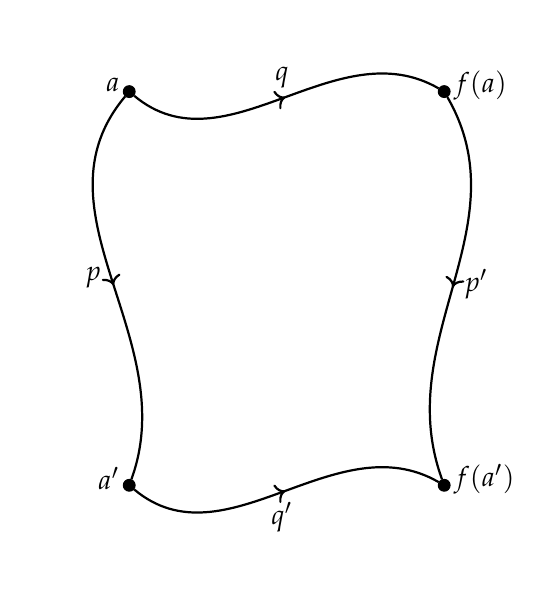
\begin{tikzpicture}
  [decoration={markings,mark=at position 0.5 with {\arrow{>}}},
   witharrow/.style={postaction={decorate}},
   dot/.style={draw,fill,circle,inner sep=1.5pt,minimum width=0pt}
  ]

    \node[dot,label={[left] $a$}] (a1) at (0,0) {};
    \node[dot,label={[left]$a'$}] (a2) at (0,-5) {};
    \node[dot,label={[right]$f(a)$}] (f1) at (4,0) {};
    \node[dot,label={[right]$f(a')$}] (f2) at (4,-5) {};
    \draw[thick,witharrow] (a1) to[out=230,in=70]node[left]{$p$} (a2);
    \draw[thick,witharrow] (a1) to[out=320,in=150]node[above]{$q$} (f1);
    \draw[thick,witharrow] (f1) to[out=300,in=110]node[right]{$p'$} (f2);
    \draw[thick,witharrow] (a2) to[out=320,in=150]node[below]{$q'$} (f2);
\end{tikzpicture}
\]
In other words, to find $p : (a = a')$, we need to find $q : (a = f(a)), q' : (f(a) = a')$, and $p' : (f(a) = f(a'))$. Setting \[g :\equiv \id_A,\] we can get the paths $q,q'$. In particular, if $h : \prod_{f : A \to A}\prod_{g : A \to A}(f = g)$, we have
\[\happly(h(f,\id_A), a') : (f(a') = a') \quad \text{and} \quad \happly(h(f,\id_A), a)^{-1} : (a = f(a))\]
To get $p' : (f(a) = f(a'))$, we could set $g$ to be the constant map $a \mt f(a')$ to get
\[\happly(h(f,a \mt f(a')),a) : (f(a) = f(a')),\] and so we can define $G$ as follows:
\[G(f,h,a,a') : \equiv \happly(h(f,\id_A), a)^{-1} \sqbullet \happly(h(f,a \mt f(a')),a) \sqbullet \happly(h(f,\id_A), a')\]


\begin{prob}{3.5}{}
Show that \[\isProp(A) \simeq (A \to \isContr(A)).\]
\end{prob}
\begin{itemize}
\item Consider the map \[F : \left(\prod_{a,a':A}(a=a')\right) \to \left(A \to \sum_{a:A}\prod_{a':A}(a=a')\right)\] defined by \[F(h,a) : \equiv (a, a' \mt h(a,a')).\]

\item Consider the map \[G : \left(A \to \sum_{a:A}\prod_{a':A}(a=a')\right) \to \left(\prod_{a,a':A}(a=a')\right)\]
defined by 
\[G(h,a,a') :\equiv \pr_2(h(a))(a')\]
\end{itemize}

We are now ready to investigate the homotopies.

\begin{itemize}
\item Consider $F \circ G \sim \id_{\left(A \to \sum_{a:A}\prod_{a':A}(a=a')\right)}$. For any function $h : \left(A \to \sum_{a:A}\prod_{a':A}(a=a')\right)$, we need to produce a path
\[F(G(h)) = h\]
Expanding the left-hand side gives us

\begin{align*}
F(G(h)) &\equiv F(a \mt a' \mt \pr_2(h(a))(a')) \\
&\equiv a \mt (a, a' \mt \pr_2(h(a))(a'))
\end{align*}
Using function extensionality, we need to provide a path
\[(a, a' \mt \pr_2(h(a))(a')) = h(a)\]
We prove a more general result (to be able to use induction on $h(a)$):
\[(a, a' \mt \pr_2(z)(a')) = z \tag{$\star$}\] for any $z : \sum_{a:A}\prod_{a':A} (a = a')$
Using induction on $z :\equiv (a,f)$, which is a sum type, it suffices to show
\[(a, a' \mt f(a')) = (a,f)\] which is judgmentally equivalent to 
\[(a, f) = (a,f),\] and the result holds by taking the witness $\refl_{(a,f)}$. Thus, plugging $h(a)$ for $z$ in $(\star)$ (technically, function elimination) gives us our path.

\item Consider $G \circ F \sim \id_{\prod_{a,a':A}(a=a')}$. For any function $h : \prod_{a,a':A}(a = a')$, we need a path: \[G(F(h)) = h.\] Observe:
\begin{align*}
G(F(h)) &\equiv G\Big(a \mt (a, a' \mt h(a,a'))\Big) \\
&\equiv a \mt a' \mt \pr_2((a,a' \mt h(a,a')))(a') \\
&\equiv a \mt a' \mt h(a,a') \\
&= h
\end{align*}
which gives us the required path using uniqueness of functions.
\end{itemize}


\begin{prob}{3.6}{}
Show that if $A$ is a mere proposition, then so is $A + (\neg A)$. Thus, there is no need to insert a propositional truncation in $3.4.1$.
\end{prob}
Since $A$ is a mere proposition, we can find an inhabitant of
\[H : \prod_{a,a':A}(a = a').\] As a bonus, note that $\neg A$ is also a mere proposition. Using function extensionality, it suffices to show
\[F : \prod_{f,g: \neg A}\prod_{a:A} (f(a) = g(a))\] and we take as a witness
\[F(f,g,a) :\equiv \rec_\0(f(a) = g(a),f(a)).\] Thus, $\neg A$ is a mere proposition with witness
\[f \mt g \mt \funext(F(f,g)) : \prod_{f,g:\neg A}(f = g)\]
Note that we are not done, as the coproduct of two mere propositions is not necessarily a mere proposition; e.g., $\1 + \1$ is not a mere proposition since $\inl(\0) \neq \inr(\0)$.\\
To prove that $A + (\neg A)$ is a mere proposition, we need to show
\[\prod_{x,y : A + (\neg A)}(x=y).\] To do this, we use double induction on the coproduct type. It suffices to provide four paths. Induction on $x: A + (\neg A)$ gives us $\inl(a),\inr(b)$ for some $a:A, b: \neg A$, and induction on $y: A + (\neg A)$ gives us $\inl(a'),\inr(b')$ for some $a':A, b': \neg A$. Now we need to produce the paths:
\begin{itemize}
\item [1)] $\inl(a) = \inl(a')$
\item [2)] $\inl(a) = \inr(b')$
\item [3)] $\inr(b) = \inl(a')$
\item [4)] $\inr(b) = \inr(b')$
\end{itemize}
It is straightforward to see that $2)$ and $3)$ are symmetric; thus, we will show $1),2),4)$.

\begin{itemize}
\item [1)] To produce $\inl(a) = \inl(a')$, recall that $A$ is a mere proposition. By path induction, we have $P : \prod_{a,a':A}(a = a') \to (\inl(a) = \inl(a'))$ (take $a \mt \refl_{\inl(a)}$ as a witness). Thus, we have \[P(H) : (\inl(a) = \inl(a')).\]

\item [2)] To produce $\inl(a) = \inr(b')$, recall that $\neg A :\equiv A \to 0$ and so we can take 
\[\rec_\0((\inl(a) = \inr(b')), b'(a)) : (\inl(a) = \inr(b'))\]
\item [3)] To produce $\inr(b) = \inl(a')$, use the same argument as in $2)$.
\item [4)] To produce $\inr(b) = \inr(b')$, recall that $\neg A$ is a mere proposition, as proved at the beginning of the problem. Thus, the same argument as in $1)$ applies. By path induction, we have $P' : \prod_{b,b' : \neg A}(f = g) \to (\inr(b), \inr(b'))$, and so
\[P'(b,b') :\equiv \funext(F(b,b')) : (\inr(b) = \inr(b'))\]
\end{itemize}
This finishes the proof.


\begin{prob}{3.7}{}
More generally, show that if $A$ and $B$ are mere propositions and $\neg(A \times B)$, then $A + B$ is also a mere proposition.
\end{prob}
We need to show 
\[P : \neg (A \times B) \to \prod_{x,y:A+B}(x = y)\]
In particular, given $h : \neg(A \times B)$, we want to produce
\[P(h) : \prod_{x,y:A+B}(x = y),\] and to do this, we use the induction principle for the sum type. We have to produce four paths, given $\inl(a),\inr(b)$ for the induction on $x : A+B$ and $\inl(a'),\inr(b')$ for the induction on $y : A+B$, where $a,a' : A$ and $b,b':B$.
\begin{itemize}
\item [1)] The first path is $\inl(a) = \inl(a')$.
The argument here is the same as the previous problem.
\item [2)] The second path is $\inl(a) = \inr(b')$. For this, observe that $h(a,b') : \0$, and so, by the induction principle for the zero type, we can conclude anything. Thus, the witness is
\[\rec_\0((\inl(a) = \inr(b')), h(a,b'))\]
\item [3)] $\inr(b) = \inl(a')$. Symmetrically, the witness is \[\rec_\0((\inr(b) = \inl(a')), h(a',b)).\]
\item [4)] $\inr(b) = \inr(b')$. The argument is the same as in the previous problem.
\end{itemize}
This finishes the proof.


\begin{prob}{3.8}{}
Assuming that some type $\isequiv(f)$ satisfies conditions $(i)-(iii)$ of $2.4$, show that the type $||\qinv(f)||$ satisfies the same conditions and is equivalent to $\isequiv(f)$.
\end{prob}
We start by recalling the definitions. For any $f : A \to B$, we have
\[\qinv(f) : \sum_{g : B \to A}((f \circ g) \sim \id_{B}) \times ((g \circ f) \sim \id_{A})\] and the propositional truncation $||A||$ of a type $A : \UU$ is a type with two constructors $c : A \to ||A||$ and $\prod_{a,a' :||A||}(a = a') $ such that the first constructor is defined by sending $a : A$ to $|a| : ||A||$.\\
The conditions $(i)-(iii)$ are:
\begin{itemize}
\item [(i)] There is a function $h : \isequiv(f) \to \qinv(f)$.
\item [(ii)] There is a function $g : \qinv(f) \to \isequiv(f)$.
\item [(iii)] For $a,b : \isequiv(f)$, we have $a = b$.
\end{itemize}

Condition $(iii)$ is satisfied by $||\qinv(f)||$ by definition of the second constructor. Now, we define the two functions $F : ||\qinv(f)|| \to \isequiv(f)$ and $G : \isequiv(f) \to ||\qinv(f)||$.\\
To define the second function, we can take
\[G :\equiv e \mt (c \circ h)(e)\]
For the first function, we use induction on $||\qinv(f)||$. We need to provide a map
\[\qinv(f) \to \isequiv(f),\] and since $\isequiv(f)$ is a mere proposition, the reasoning makes sense. But this is just $g : \qinv(f) \to \isequiv(f)$, and so
\[F :\equiv a \mt \rec_{||\cdot||}(\isequiv(f),g)\]

It remains to show the two homotopies.

\begin{itemize}
\item Consider $F \circ G \sim \id_{\isequiv(f)}$. We need to show
\[F(G(e)) = e\] for any $e : \isequiv(f)$. Since $F$ takes its argument to an element of $\isequiv(f)$ and $\isequiv(f)$ is itself a mere proposition, the equation is verified by $(iii)$.

\item Consider $G \circ F \sim \id_{\qinv(f)}$. We need to show
\[G(F(e)) = e\] for any $e : ||\qinv(f)||$. Similarly, since $G$ takes its argument to a mere proposition, the equation is verified by induction on $e : ||\qinv||$. More precisely, induction on $e :\equiv |e|$ gives us
\[G(F(|e|)) = |e|,\] and since $G(F(|e|)) : ||\qinv(f)||$, the constructor of truncation gives us $G(F(|e|)) = |e|$.
\end{itemize}

\begin{prob}{3.9}{}
Show that if LEM holds, then the type $\text{Prop} :\equiv \sum_{A:\UU} \isProp(A)$ is equivalent to $\2$.
\end{prob}
We wish to show:
\[L : \left(\prod_{A:\UU}\isProp(A) \to (A + (\neg A)) \right) \to \left(\sum_{A : \UU}\isProp(A) \simeq 2 \right)\]
where \[\isProp(A) :\equiv \prod_{a,a':A}(a = a')\]

Define the map $h : (A + (\neg A)) \to \2$ by recursion:
\[h :\equiv \rec_{A + \neg A}(\2, 0_\2, 1_\2).\] Now, given a map $f : \left(\prod_{A:\UU}\isProp(A) \to (A + (\neg A)) \right)$, we would like to produce an equivalence $\left(\sum_{A : \UU}\isProp(A) \simeq 2 \right)$.
\[L(f) : \left(\sum_{A : \UU}\isProp(A) \simeq 2 \right)\] The forward map $F : \left(\sum_{A : \UU}\isProp(A) \to 2 \right)$ is defined by recursion on the sum type $\sum_{A : \UU}\isProp(A)$. It suffices to consider $(A,p) :\sum_{A : \UU}\isProp(A)$ and
\[(A,p) \mt h(f(A,p)),\] so that the map is
\[F : \equiv \rec_{\sum}(\2,A \mt p \mt h(f(A,p)))\]
For the reverse map $G : \2 \to \sum_{A:\UU}\isProp(A)$, by recursion on $\2$, we need to generate a tuple $(A,p)$ consisting of a type $A : \UU$ and a proof $p:\isProp(A)$ that it is a proposition for $0_\2$ and $1_2$. We know that $\0$ and $\1$ are mere propositions, so we can define the map as
\[G :\equiv \rec_\2((\1,p_\1), (\0,p_\0)),\] where $p_\0 : \isProp(\0)$ and $p_\1 : \isProp(\1)$. (These are straightforward to prove by induction on the respective types. We believe an argument is provided in the book as well.)\\
Now, let us consider the homotopies.

\begin{itemize}
\item For $F \circ G \sim \id_{\2}$, we need to show $F(G(x)) = x$ for any $x : \2$. By induction on $x : \2$, it suffices to provide two paths:
\[F(G(0_\2)) = 0_\2 \quadt{and} F(G(1_\2)) = 1_\2.\] Unraveling the definitions:
\begin{align*}
F(G(0_\2)) &\equiv F((\0, p_\0)) \\
&\equiv h(f(\0, p_\0)) \\
&\equiv \rec_{\0 + \neg \0}(\2, 0_\2, 1_\2, \0) \\
&\equiv 0_\2 \\
\end{align*}
Since the type $\0$ is decidable, our witness is $\refl_{0_\2}$. Similarly, the other path will lead to the witness $\refl_{1_\2}$ since $\1$ is decidable.

\item For $G \circ F \sim \id_{\sum_{A:\UU}\isProp(A)}$, we need to show
\[G(F(x)) = x,\] and by recursion on the sum type, it suffices to show
\[G(F(A,p)) = (A,p)\] for any $A : \UU$ and $p : \isProp(A)$. We observe:

\begin{align*}
G(F(A,p)) &\equiv G(h(f(A,p))) \\
\end{align*}
By induction on $f(A,p) : A + \neg A$, we need to consider two cases:
\[G(h(A)) \quadt{and} G(h(\neg A)).\] In the first case, we have $h(A) \equiv 0_\2$, and so $G(h(A)) \equiv (\1,p_\1)$. We thus need to find
\[(\1,p_\1) = (A,p),\] but since $A$ is a mere proposition, it is equivalent to $\1$, and $\Prop$ is a mere proposition as well; thus, $p_\1 \simeq p$. By univalence, we can now extract a path from the equivalences. The other path is similar.

\end{itemize}
 
\begin{prob}{3.10}{}
Show that if $\UU_{i+1}$ satisfies LEM, then the canonical inclusion $\text{Prop}_{\UU_i} \to \text{Prop}_{\UU_{i+1}}$ is an equivalence.
\end{prob}
Recall the definition of $\Prop_{\UU_i}$:
\[\Prop_{\UU_i}:\equiv \sum_{A : U_i}\isProp(A).\] We need to define the reverse map $G : \Prop_{\UU_{i+1}} \to \Prop_{\UU_i}$. Since $\UU_{i+1}$ satisfies LEM, given $A : \UU_{i+1}$, we can decide between $A$ and $\neg A$. In the first case, we can resize $A$ to be $\1 : \UU_i$, and in the second case, $\0 : \UU_i$. Call the corresponding proofs $p_0 : \isProp(\0)$ and $p_1 : \isProp(\1)$, respectively. Define the map $\mathrm{Decide} : A \to \sum_{B:\UU_i} \isProp(B)$ by
\[\mathrm{Decide}(A) :\equiv \Big(\rec_{A + \neg A}(\1,\0,\LEM(A)), \rec_{A + \neg A}(p_1,p_0,\LEM(A))\Big).\] This map basically returns $(\1,\isProp(1)$ if $A$ holds or $(\0,\isProp(0))$ if $\neg A$ holds. We are now ready to define the map $G: \Prop_{\UU_{i+1}} \to \Prop_{\UU_i}$ as
\[G(x) :\equiv \rec_{\sum_{A : U_{i+1}}\isProp(A)}\left(\sum_{A : U_i}\isProp(A),A \mt p \mt \mathrm{Decide}(A) ,x\right).\]
Together with the inclusion map $F : \Prop_{\UU_i} \to \Prop_{\UU_{i+1}}$, defined as $x \mt x$, we can investigate the homotopies.

\begin{itemize}
\item Consider $F \circ G \sim \id_{\Prop_{\UU_{i+1}}}$. We need to prove
\[F(G(x)) = x \quad \text{for some } x : \sum_{A : \UU_{i+1}}\isProp(A).\] The left-hand side reduces to
\begin{multline*}
F\left(\rec_{\sum_{A : U_{i+1}}\isProp(A)}\left(\sum_{A : U_i}\isProp(A),A \mt p \mt \mathrm{Decide}(A) ,x\right)\right) \\
\equiv \rec_{\sum_{A : U_{i+1}}\isProp(A)}\left(\sum_{A : U_i}\isProp(A),A \mt p \mt \mathrm{Decide}(A) ,x\right)
\end{multline*}
Now, using induction on the sum type, we consider $x \equiv (A,b)$, and so we need to show
\[\rec_{\sum_{A : U_{i+1}}\isProp(A)}\left(\sum_{A : U_i}\isProp(A),A \mt p \mt \mathrm{Decide}(A) ,(A,b)\right)\] which reduces to 
\[\mathrm{Decide}(A).\]
\item 
\end{itemize}
%TODO to finish

\begin{prob}{3.11}{}
Show that it is not the case that, for all $A : \UU$, we have $||A|| \to A$. (However, there can be particular types for which this is true, e.g., $\qinv(f)$.)
\end{prob}
This problem uses an argument almost identical to the proof of \[\left(\prod_{A : \UU} \neg \neg A \to A \right) \to 0\] in the text. The idea is similar, but instead of using the fact that all elements of $\neg \neg A$ are propositionally equal, we will use the fact that all elements of $||A||$ have the same property \textbf{by definition}.\\
Assume that we are given a function \[f : \prod_{A:\UU} ||A|| \to A.\] We would like to produce an element of $\0$. To do this, take the equivalence $e : \2 \simeq \2$ such that $e(0) \equiv 1$ and $e(1) \equiv 0$, with the abuse of notation $e(0) :\equiv \pr_1(e)(0)$. By univalence, we get a path $p : \2 = \2$. We now use this path to transport $f(\2)$ along the type family $A \to ||A|| \to A$ to produce another function $\tr^{A \to ||A|| \to A}(p,f(\2)) : ||\2|| \to \2$. By the definition of transport, we have a path.
\[f(\2) = \tr^{A \to ||A|| \to A}(p,f(\2))\]
Since functions preserve paths, for any $u : ||\2||$, we have
\[f(\2)(u) = \tr^{A \to ||A|| \to A}(p,f(\2))(u)\]
Recall that transporting a function (here $f(\2) : ||\2|| \to \2$) and evaluating it at $u : ||\2||$ is the same (propositionally equal) as first transporting the argument, applying the function, and transporting the result back. Thus, we have
\[\tr^{A \to ||A|| \to A}(p,f(\2))(u) = \tr^{A \to A}(p,f(\2)(\tr^{A \to ||A||}(p^{-1}, u)))\]
Now, notice that $\tr^{A \to ||A||}(p^{-1}, u) : ||\2||$, and by the definition of truncation, since $u : ||\2||$, they are equal.
\[\tr^{A \to ||A||}(p^{-1}, u) = u.\] Thus, the previous path becomes
\[\tr^{A \to ||A|| \to A}(p,f(\2))(u) = \tr^{A \to A}(p,f(\2)(u)),\] and thus, combining it with our previous path,
\[\tr^{A \to A}(p,f(\2)(u)) = f(\2)(u)\]
Finally, note that $\tr^{A \to A}(p,f(\2)(u)) : \2$, and so transporting with a path generated by an equivalence is the same as evaluating at the equivalence. Thus,
\[\tr^{A \to A}(p,f(\2)(u)) = e(f(\2)(u)),\] which leads to the final path:
\[e(f(\2)(u)) = f(\2)(u)\]
Now, our choice of equivalence will generate a contradiction (i.e., an element of $\0$). This is because, in the type $\2$, we do not have any path between $0_\2 : \2$ and $1_\2 : \2$. In particular,
\[H : \left(\prod_{x,y:\2} (x=y) \right) \to \0.\] Once we prove that this type is inhabited, we will take $x :\equiv e(f(\2)(u))$ and $y : \equiv f(\2)(u)$ to generate an element of $\0$, namely, $H(e(f(\2)(u)),f(\2)(u)) : \0$.\\
It remains to show that $\left(\prod_{x,y:\2} (x=y) \right) \to \0$ is inhabited. Given a function $h : \prod_{x,y:\2} (x=y)$, we need to produce an element of $\0$. To do this, observe that
\[h(0_\2, 1_\2) : (0_\2 = 1_\2),\] but $(0_\2 = 1_\2) \to \0$ is inhabited (cf. the Useful Results section), which provides the result.\\



\begin{prob}{3.12}{}
Show that if LEM holds, then for all $A : \UU$, we have $||(||A|| \to A)||$. (This property is a very simple form of the axiom of choice, which can fail in the absence of LEM.)
\end{prob}
We have to be careful not to try to prove
\[\left(\prod_{A:\UU}\isProp(A) \to (A + (\neg A)) \right) \to \prod_{A:\UU} ||(||A|| \to A)||\]
which is clearly not inhabited (e.g., when $A$ is not a mere proposition). Instead, we would like to show:
\[F : \prod_{A:\UU}\isProp(A) \to \Big((A + (\neg A)) \to ||(||A|| \to A)|| \Big)\]
Given a type $A:\UU$, a proof that it is a mere proposition $P : \isProp(A)$, and an element $l : A + (\neg A)$, we wish to produce an element \[F(A,P,l) : ||(||A|| \to A)||.\] By recursion on $l : A + \neg A$, we need to provide two maps:
\[A \to ||(||A|| \to A)|| \quad \text{and} \quad \neg A \to ||(||A|| \to A)||\]
Now, by the definition of truncation, we only need to produce an element of $||A|| \to A$, and finally, by induction on truncation, we want two maps:
\[A \to (A \to A) \quad \text{and} \quad \neg A \to (A \to A)\]
The first map is witnessed by $a \mt \id_{A}$, and the second is witnessed by $a \mt \rec_\0(A \to A,a)$.


\begin{prob}{3.13}{}
We showed in Corollary $3.2.7$ that the following naive form of LEM is inconsistent with univalence: \[\LEM_{\infty} : \prod_{A:\UU}(A + (\neg A)).\] In the absence of univalence, this axiom is consistent. However, show that it implies the axiom of choice $(3.8.1)$.
\end{prob}
The axiom of choice is 
\[\AC :\equiv \prod_{x : X} \left| \left|\sum_{a:A(x)} P(x,a) \right|\right| \to \left| \left| \sum_{g:\prod_{x:X}A(x)} \prod_{x:X} P(x,g(x)) \right|\right|\]
Given $h : \prod_{A:\UU}(A + (\neg A))$, we would like to show that $\AC$ holds. Thus, we want to produce
\[\AC(f) : \left| \left| \sum_{g:\prod_{x:X}A(x)} \prod_{x:X} P(x,g(x)) \right|\right|\] for any $f : \prod_{x : X} \left| \left|\sum_{a:A(x)} P(x,a) \right|\right|$. Recall that we have the equivalence
\[\left(\prod_{x : X} \sum_{a:A(x)} P(x,a) \right) \simeq \left(\sum_{f : \prod_{x:X}A(x)} \prod_{x:X}P(x,f(x)) \right),\] and since only one direction is provided in the useful result (namely, the reverse direction), we provide the forward direction here:
\[g \mt (x \mt (\pr_1 \circ g)(x), x \mt (\pr_2 \circ g)(x))\] The text provides the homotopies in Theorem $2.15.7$.\\ 
Thus, our problem reduces to exhibiting an element of
\[\left| \left|\prod_{x:X}\sum_{a:A(x)}P(x,a)\right| \right|,\] and to do this, it suffices to show
\[\prod_{x:X}\sum_{a:A(x)}P(x,a).\] Since this type is not a mere proposition in general, we cannot use the induction principle as presented in the text. Instead, to guarantee that the construction will not depend on the particular choice of tuples $(x,a) : \prod_{x:X}\sum_{a:A(x)}P(x,a)$, we will show that all our proofs are propositionally equal. To be precise, to find a function
\[\left| \left|\prod_{x:X}\sum_{a:A(x)}P(x,a)\right| \right| \to \prod_{x:X}\sum_{a:A(x)}P(x,a)\] it is natural to think of taking
\[|(a,b)| \mt (a,b).\] But this is not allowed since the result depends on the inputs. Namely, we do not have $(a,b) = (a,b')$ for any $a,a':A$ and $b:B(a), b':B(a')$; it is even worse since $B(a)$ and $B(a')$ are not even required to be the same type in general. Instead, we construct a function such that the result will be independent of the input. To do this, we will need $\LEM_{\infty}$. \\
To simplify the problem, we show that if $C$ is decidable in the sense of $\LEM_{\infty}$, then we have a function $||C|| \to C$. Then, replacing $C$ by $\prod_{x:X}\sum_{a:A(x)}P(x,a)$ leads to the result.\\
More precisely, we want
\[(C + \neg C) \to ||C|| \to C.\] By recursion on the sum type, it suffices to produce
\[C \to ||C|| \to C \quadt{and} \neg C \to ||C|| \to C.\] The first function is simply
\[c \to |c| \to c.\] We need to work a little more on the second function. We define it as
\[b \mt |c| \mt \rec_\0(C,b(c)).\] The critical point is that we need to check that
$\rec_\0(C,b(c)) = \rec_\0(C,b(c'))$ for any $c,c'$, to guarantee that the result is independent of the particular $c:C$ we used. To do this, consider the map
\[\rec_\0(C,-) : \0 \to C\] defined by $x \mt rec_\0(C,x)$. We would like to show that
\[\prod_{x,x':\0}\rec_\0(C,x) = \rec_\0(C,x') \tag{$\star$}\] and we will be finished, since substituting $b(c)$ for $x$ and $b(c')$ for $x'$ gives us the result. We have two ways of showing $(\star)$. The first consists of observing that, since $x:\0$, we can deduce anything by induction on it.\\
A second way to see that this holds is to prove that $p : (x = x')$, also using induction on $x,x':\0$, and then take $\ap_{\rec_\0(C,-)}(p)$.


\begin{prob}{3.14}{}
Show that, assuming LEM, the double negation $\neg \neg A$ has the same recursion principle as the propositional truncation $||A||$, but with a propositional computation rule rather than a judgmental one. \\
In other words, prove that, assuming LEM, if $B$ is a mere proposition and we have $f : A \to B$, then there is an induced $g : \neg \neg A \to B$ such that $g(|a|) = f(a)$ for all $a : A$. \\
Deduce that, assuming LEM, we have $\neg \neg A \simeq ||A||$. Thus, under LEM, the propositional truncation can be defined rather than taken as a separate type former.
\end{prob}
%TODO TO FINISH
Note: We can also prove the equivalence directly, assuming that $A$ is a proposition, as follows. Recall that to prove
\[\neg \neg A \simeq ||A||\]
we only need to show the logical equivalence
\[\neg \neg A \leftrightarrow ||A||,\] since both types are propositions (i.e., all paths will be inhabited).
We then define the forward and reverse maps, respectively, as
\[b \mt |h(b)| \quadt{and} |a| \mt \rec_{||\cdot||}(\neg \neg A,G(a)),\] where $h : \neg \neg A \to A$ is double-negation elimination (available because of LEM), and $G : A \to \neg \neg A$ is double-negation introduction, available without assuming LEM.\\
A few words are needed here. First, let us define double-negation elimination assuming LEM, i.e.,
\[h : \neg \neg A \to A\]
Since $\neg \neg A$ is a proposition, we need to consider two cases: either $A:\UU$ or $\neg A : \UU$ is inhabited. In the former case, the identity map is enough. In the latter case, a contradiction arises.\\
Finally, $|a| \mt \rec_{||\cdot||}(\neg \neg A,G(a))$ is well-defined since $\neg \neg A$ is a proposition (this is true without assuming that $A$ is a proposition).


\begin{prob}{3.15}{}
Show that if we assume propositional resizing as in $3.5$, then the type \[\prod_{P : \Prop} \Big((A \to P) \to P \Big)\] has the same recursion principle as $||A||$, with the same judgmental computation rule. Thus, we can also define the propositional truncation in this case.
\end{prob}
We would like to find out how to define a map 
\[\prod_{P : \Prop} \Big((A \to P) \to P \Big) \to C\] for any type $C : \UU$. Assume propositional truncation $\Prop_{\UU_i} \simeq \Prop_{\UU_{i+1}}$.

\begin{prob}{3.16}{}
Assuming LEM, show that double negation commutes with universal quantification of mere propositions over sets. That is, show that if $X$ is a set and each $Y(x)$ is a mere proposition, then LEM implies
\[\left(\prod_{x:X} \neg \neg Y(x)\right) \simeq \left(\neg \neg \prod_{x:X} Y(x)\right)\]
Observe that, if we assume instead that each $Y(x)$ is a set, then $3.11.11$ becomes equivalent to the axiom of choice $3.8.3$.
\end{prob}
We start by defining the two maps:
\begin{align*}
F : \left(\prod_{x:X} \neg \neg Y(x)\right) &\to \left(\neg \neg \prod_{x:X} Y(x)\right)  \\
G :  \left(\neg \neg \prod_{x:X} Y(x)\right) &\to \left(\prod_{x:X} \neg \neg Y(x)\right)
\end{align*}

\begin{itemize}
\item To define $F$, suppose we are given a map $f : \prod_{x:X} \neg \neg Y(x)$ and a map $g : \prod_{x:X} Y(x) \to \0$. We would like to produce an element of $\0$. Take:
\[F(f,g):\equiv f(g)\]
\item To define $G$, suppose we are given a map $f : \neg \neg \prod_{x:X} Y(x)$, $x : X$, and $g: Y(x) \to \0$. We would like to produce an element of $\0$.
\[G(f,x,g) : \equiv \]
\end{itemize}

\begin{prob}{3.17}{}
Show that the rules for the propositional truncation given in $3.7$ are sufficient to imply the following induction principle: for any type family $B : ||A|| \to \UU$ such that each $B(x)$ is a mere proposition, if for every $a:A$ we have $B(|a|)$, then for every $x : ||A||$, we have $B(x)$.
\end{prob}

\begin{prob}{3.18}{}
Show that the law of excluded middle $3.4.1$ and the law of double negation $3.4.2$ are logically equivalent.
\end{prob}
We need to show 
\[\left(\prod_{A:\UU}\isProp(A) \to (A + \neg A) \right) \simeq \left(\prod_{A:\UU}\isProp(A) \to (\neg \neg A \to A)\right).\] Call $F$ and $G$ the forward and reverse maps, respectively. Define \[F : \left(\prod_{A:\UU}\isProp(A) \to (A + \neg A) \right) \to \left(\prod_{A:\UU}\isProp(A) \to (\neg \neg A \to A)\right)\] by
\[F(f,A,p,b) : \equiv \rec_{A + \neg A}(A,\id_A, c \mt \rec_\0(A,b(c)), f(A,p))\]
Informally, if $f(A,p) : A + \neg A$ is an element of $A$, then the map $\id_A$ works for $A \to \neg \neg A \to A$. If $f(A,p)$ is an element of $\neg A$, then for the map $\neg A \to \neg \neg A \to A$ we can take $c \mt b \mt \rec_\0(A, b(c))$.\\
Now, for the reverse map,
\[G : \left(\prod_{A:\UU}\isProp(A) \to (\neg \neg A \to A)\right) \to \left(\prod_{A:\UU}\isProp(A) \to (A + \neg A) \right)\]
we need to think a little more. We can take inspiration from logic and from how to derive the law of excluded middle from double-negation elimination. Here is one way to do it:

\begin{prooftree}
     \AxiomC{}
     \RightLabel{\scriptsize(1)}
     \UnaryInfC{$\neg \neg A \to A$}
     \AxiomC{}
     \RightLabel{\scriptsize(2)}
     \UnaryInfC{$\neg (A \vee \neg A)$}
     \AxiomC{}
     \RightLabel{\scriptsize(3)}
     \UnaryInfC{$A$}
     \UnaryInfC{$A \vee \neg A$}
     \BinaryInfC{$\bot$}
     \RightLabel{\scriptsize(3)}
     \UnaryInfC{$\neg A$}
	  \UnaryInfC{$A \vee \neg A$}
	  \RightLabel{\scriptsize(2)}
	  \UnaryInfC{$\neg \neg (A \vee \neg A)$}
	  \RightLabel{\scriptsize(1)}
     \BinaryInfC{$(\neg \neg A \to A) \to (A \vee \neg A)$}
\end{prooftree}

From this, we get the idea of defining the trivial injection maps
\[\inl_A : A \to A + \neg A \quad \text{and} \quad \inr_{\neg A} : \neg A \to A + \neg A,\] where $\inl_{-}$ and $\inr_{-}$ are merely suggestive notation: $\inl_A(a) :\equiv \inl(a)$ and $\inr_{\neg A}(a) :\equiv \inr(a)$. Now, define $G$ as follows:
\[G(f,A,p) : \equiv f(A + \neg A,p'(p),H),\] where $p'(p) :\isProp(A + \neg A)$ is a proof that $A + \neg A$ is a proposition, given that $A$ is one (i.e., Problem $3.7$), and $H : \neg \neg (A + \neg A)$, so that the result is an element of $A + \neg A$. We define $H$ to be
\[H(b) : \equiv b(\inr_{\neg A}( a \mt b(\inl_A(a)))\]
Take a moment to check whether this type-checks and whether the result follows from our natural deduction.


\begin{prob}{3.19}{}
Suppose $P : \N \to \UU$ is a decidable family ($3.4.3(ii)$) of mere propositions. Prove that 
\[\left|\left|\sum_{n : \N}P(n) \right| \right| \to \sum_{n:\N}P(n)\]
\end{prob}
A more general version is proved in $3.23$.

\begin{prob}{3.20}{}
Prove Lemma $3.11.9(ii)$: If $A$ is contractible with center $a$, then $\sum_{x : A}P(x)$ is equivalent to $P(a)$.
\end{prob}
Recall the definition of contractibility:
\[\isContr(A) : \sum_{a:A}\prod_{a':A}a = a'\]
We need to show
\[\sum_{x:A}P(x) \simeq P(a),\] knowing that $A$ is contractible with center $a$, or, more precisely,
\[H : \prod_{A:\UU} \prod_{c:\isContr(A)} \left(\sum_{x:A}P(x) \simeq P(\pr_1(c)) \right)\]
We have
\[H(A,c) : \sum_{x:A}P(x) \simeq P(\pr_1(c)).\] We start with the forward direction $F : \sum_{x:A}P(x) \to P(\pr_1(c))$. We define the map by induction on the sum type:
\[F(a,b) :\equiv T(a,\pr_1(c),b)\] where $T : \prod_{x,y:A}(x = y) \to P(x) \to P(y)$ is defined as 
\[T :\equiv \rec_{=}(E,x \mt \id_{P(x)})\] for the family $E : \prod_{a,a':A} P(x) \to P(y)$. Thus, our map is
\[F :\equiv \rec_{\sum}\Big(P(\pr_1(c)), a \mt b \mt T(a,\pr_1(c),b)\Big),\] or, in a more formal and verbose form,
\[F :\equiv \rec_{\sum}\Big(P(\pr_1(c)), a \mt b \mt \rec_{=}(E,x \mt \id_{P(x)}a,\pr_1(c))(b)\Big)\]
For the reverse map, define $G : P(\pr_1(c)) \to \sum_{x:A}P(x)$ by 
\[G(b): \equiv (\pr_1(c),b),\] and we now check the homotopies.

\begin{itemize}
\item Consider $F \circ G \sim \id_{P(\pr_1(c))}$. We need to show 
\[F(G(b)) = b\] for any $b : P(\pr_1(c))$. Expanding the left-hand side gives
\begin{align*}
F(G(b)) &\equiv F((\pr_1(c),b)) \\
&\equiv \rec_{\sum}\Big(P(\pr_1(c)), a \mt b \mt T(a,\pr_1(c),b)\Big)(\pr_1(c),b) \\
&\equiv T(\pr_1(c),\pr_1(c),b)\\
&\equiv \rec_{=}(E,x \mt \id_{P(x)})(\pr_1(c),\pr_1(c), \refl_{\pr_1(c)})(b)\\
&\equiv \id_{\pr_1(c)}(b)\\
&\equiv b
\end{align*}
Thus, we can take $\refl_b$ as a witness.

\item Consider $G \circ F \sim \id_{\sum_{x:A}P(x)}$. We need to show 
\[G(F(b)) = b\] for any $b : \sum_{x:A}P(x)$. By induction on the sum type, it suffices to show
\[G(F((r,s)) = (r,s)\] for some $r : A$ and $s : P(r)$.
Expanding the left-hand side gives

\begin{align*}
G(F((r,s)) &\equiv T(r,\pr_1(c),s) \\
&\equiv G(\rec_{=}(E,x \mt \id_{P(x)})(r,\pr_1(c), \pr_2(\isContr(A))(r))(s)) \\
\end{align*}
By based path induction on $r,\pr_1(c) : A$ and $\pr_2(\isContr(A))(r) : (r = \pr_1(c))$, it suffices to consider $\pr_1(c) : A$ and $\refl_{\pr_1(c)}$.

\[
\rec_{=}(E,x \mt \id_{P(x)})(r,\pr_1(c), \pr_2(\isContr(A))(r))(s) \]
which is equivalent to   
\begin{align*}
\rec_{=}(E,x \mt \id_{P(x)})(\pr_1(c),\pr_1(c), \refl_{\pr_1(c)})(s)
&\equiv \id_{P(x)}(s)\\
&\equiv s
\end{align*}
and so \[G(F((r,s)) \equiv G(s) \equiv (\pr_1(c),s)\] and since $A$ is contractible with center $\pr_1(c)$, we have $\pr_1(c) = r$, which leads to
\[(\pr_1(c),s) = (r,s)\]

\end{itemize}

\begin{prob}{3.21}{}
Prove that \[\isProp(P) \simeq (P \simeq ||P||).\]
\end{prob}
Let us denote by $c : \prod_{p,p' : ||P||} (p = p')$ the constructor of the type $||P||$ that constructs a path between two elements of $||P||$.\\
We need to provide two maps:
\[F : \isProp(P) \to (P \simeq ||P||) \quadt{and} G : (P \simeq ||P||) \to \isProp(P)\]
To define $F$, we need to find an equivalence $P \simeq ||P||$. The forward map is clear enough: it is $p \mt |p|$. The reverse map can be defined by induction on $||P||$ since $P$, the codomain of the map, is a mere proposition (i.e., we have a proof of $\isProp(P)$). The map is then defined as $\id_{P}$. For the homotopy $\eta : F \circ G \sim \id_{||P||}$, we note that
\[F(G(p)) = p.\] By induction on $p:||P||$, we can assume that $p$ is of the form $|p|$. Thus, $F(G(|p|)) = |p|$, and unraveling the definitions of $F,G$, we need a witness of $|p| = |p|$, which is just $\refl_{|p|}$.\\
For the homotopy $\gamma : G \circ F \sim \id_{P}$, we need \[G(F(p)) = p.\] Similarly, unraveling the definition, we need $p = p$, which is just $\refl_p$.
Thus, the equivalence is
\[(p \mt |p|, \rec_{||\cdot||}(P,\id_{P}), \eta, \gamma).\] Thus, the final map is
\[F(s) :\equiv (p \mt |p|, \rec_{||\cdot||}(P,\id_{P}), \eta, \gamma)\]
To define the reverse map, suppose we are given an equivalence $e : P \simeq ||P||$ and two elements $p,p':P$. We want to exhibit a path $p = p'$. First, by recursion on $e:P \simeq ||P||$, we can assume that $e$ is of the form $(f,g,\eta,\gamma)$, where $f : P \to ||P||$, $g : ||P|| \to P$,
$\eta : f \circ g \sim \id_{||P||}$ and $\gamma : g \circ f \sim \id_{P}$.\\
We can define it to be \[(\ap_{\eta} \circ \ap_{g})(c(f(p), f(p'))) : (p = p')\]
First, we check that the type is correct. Recall that $f(p),f(p') : ||P||$; then we get $c(f(p), f(p')) : (f(p) = f(p'))$, and finally, \[\ap_{g}(c(f(p), f(p'))) : \Big((f\circ g)(p) = (f\circ g)(p')\Big).\] Now recall that
\[\eta : \prod_{p:||P||} (f \circ g)(p) = p,\] and so \[\ap_\eta\Big(\ap_{g}(c(f(p), f(p')))\Big) : (p = p'),\] which is the type we wanted.\\
We now need to compute both homotopies.

\begin{itemize}
\item Consider $F \circ G \sim \id_{P \simeq ||P||}$; thus, we want
\[F(G(e)) = e.\] By induction on $e : P \simeq ||P||$, we can assume that $e$ is of the form $(f,g,\eta,\gamma)$. Then, by definition, we have
\begin{align*}
F(G((f,g,\eta,\gamma))) &\equiv F((\ap_{\eta} \circ \ap_{g})(c(f(p), f(p')))) \\
&\equiv F(p,p',(\ap_{\eta} \circ \ap_{g})(c(f(p), f(p')))) \\
\end{align*} 
%TODO TO FINISH
\item Consider $G \circ F \sim \id_{\isProp(P)}$; thus, we want
\[F(G(f)) = f,\] and by function extensionality, we only need to prove, for any $p,p' : P$, that
\[F(G(f))(p,p') = f(p,p')\]
\end{itemize}


\begin{prob}{3.22}{}
As in classical set theory, the finite version of the axiom of choice is a theorem. Prove that the axiom of choice $3.8.1$ holds when $X$ is a finite type $\text{Fin}(n)$ (as defined in Exercise $1.9$).
\end{prob}

\begin{prob}{3.23}{}
%TODO Lots of mistakes here
Show that the conclusion of Exercise $3.19$ is true if $P : \N \to \UU$ is any decidable family.
\end{prob}
Informally, the idea of this problem is to construct an element of $\sum_{n:\N}P(n)$ knowing only that the type is merely inhabited. In this specific case, it is possible to construct such an object due to the least-element property of the natural numbers, provided that $\LEM$ holds. This means that if we know that the type is merely inhabited, then we can always look for the least $n:\N$ that satisfies $P(n)$. In other words, given \[|(n,b)| : \left|\left|\sum_{n:\N}P(n)\right|\right|,\] we can find the least $m \leq n$ such that $P(m)$ holds. Thus, if we send $|(n,b)|$ to this least element, we are essentially done once we observe that this element is independent of the chosen $n:\N$.\\
Our strategy is then to define $\text{Least} : \N \to \2 \times \N$, where the Boolean represents whether the least element has been found (i.e., $0_\2$ if it has not been found and $1_\2$ if it has), and the natural number in the codomain records the index of the least element $m:\N$ satisfying $P(m)$. With this function in hand, we would then like to prove that \[\prod_{n,m:\N}\Big(P(n)\times P(m)\Big) \to \Big(\text{Least}(n) = \text{Least}(m)\Big),\] which will guarantee that the property captured by $\text{Least}$ is independent of the witness.\\
First, let us call the decidability function
\[\LEM_P : \prod_{n:\N} (P(n) + \neg P(n)).\]
Define $\text{Least} : \N \to \2 \times \N$ by recursion on $\N$:
\[\text{Least}(0) : \equiv \rec_{P(0)+\neg P(0)}(\2 \times \N, (1_\2, 0),(0_\2, 0), \LEM_P(0)).\]
For the base case, if $P(0)$ holds, then we return $(1_\2, 0) : \2 \times \N$, where the first entry says that we have found the least element and the second entry is its index. In the induction case, we will simply return this element.\\
If $\neg P(0)$, then we return $(0_\2, 0)$, indicating that the least element has not been found; the second entry no longer matters. The induction case will then test whether $P(\su(n))$ holds and return the correct tuple.\\
Now that the base case is covered, we define a function $c_s : \N \to (\2 \times \N) \to (\2 \times \N)$ that computes a tuple given the previous one. Recall that if the previous tuple's first entry is $1_\2$, there is nothing to be done. We use the shorthand $s_1,s_2$ to denote $\pr_1(s),\pr_2(s)$, respectively, as well as $n+1$ to denote $\su(n)$. Define $c_s$ as
\begin{multline*}
c_s(n,s) :\equiv \\ 
\rec_{\2}\Big(\2 \times \N,\rec_{P(n+1) + \neg P(n+1)}(\2 \times \N,a \mt (1_\2,n+1),a \mt (0_\2,n+1),\LEM_P(n+1)),s,s_1\Big),
\end{multline*}
and, finally, our function is defined as
\[\text{Least} : \rec_\N(\2 \times \N,\text{Least}(0),c_s).\]
Let us take a moment to unpack the definition and understand what is going on. Suppose that $P(1)$ and $P(2)$ hold, but $P(0)$ does not (i.e., $\neg P(0)$). Let us compute $\text{Least}(2)$ and $\text{Least}(1)$. Note that $\text{Least}(0) \equiv (0_\2,0)$.

\begin{align*}
\text{Least}(1) &\equiv c_s(0,\text{Least}(0)) \\
&\equiv c_s(0,(0_\2,0)) \\
&\equiv \rec_{\2}\Big(\2 \times \N,\rec_{P(1) + \neg P(1)}(\2 \times \N,a \mt (1_\2,1),a \mt (0_\2,1),\LEM_P(1)),(0_\2,0),0_\2\Big) \\
&\equiv \rec_{P(1) + \neg P(1)}(\2 \times \N,a \mt (1_\2,1),a \mt (0_\2,1),\LEM_P(1)) \\
&\equiv (1_\2,1)\\
\end{align*}
This means that the least is attained at index $n \equiv 1$. Now,
\begin{align*}
\text{Least}(2) &\equiv c_s(1,\text{Least}(1)) \\
&\equiv c_s(1,(1_\2,1)) \\
&\equiv \rec_{\2}\Big(\2 \times \N,\rec_{P(2) + \neg P(2)}(\2 \times \N,a \mt (1_\2,2),a \mt (0_\2,2),\LEM_P(2)),(1_\2,1),1_\2\Big) \\
&\equiv (1_\2,1)
\end{align*}
As expected, this returns the least element $n \equiv 1$. Note also that we get $\text{Least}(1) = \text{Least}(2)$ since $\text{Least}(1) \equiv \text{Least}(2)$.\\
Now, to finish, define the map $F : \left|\left|\sum_{n : \N}P(n) \right|\right| \to \sum_{n : \N}P(n)$ to be 
\[F :\equiv \rec_{||\cdot||}(\sum_{n : \N}P(n),g),\] where $g : \sum_{n : \N}P(n) \to \sum_{n : \N}P(n) $ is defined as
\[g : \equiv \rec_{\sum_{n : \N}P(n)}\left(\sum_{n : \N}P(n),n \mt p \mt (\text{Least}(n),P(n))\right).\]
Using the recursion principle on the truncation is justified only if the codomain type is a mere proposition. However, this assumption does not hold in our case. It is justified if our targeted values behave like a mere proposition, i.e., if all elements are equal to each other. It remains to show that
\[\prod_{n,m :\N} F(n) = F(m).\] By induction on the natural numbers, it suffices to provide four paths. Before we do, let us prove the following useful fact:
\[\prod_{n:\N} F(|(n,p_n)|) = F(|(n+1,p_{n+1})|).\] To show this by induction on $n : \N$, first consider $F(|(0,p_0)|) = F(|(1,p_1)|)$. Unraveling the definitions, we need to show $(\text{Least}(0),p_0) = (\text{Least}(1),p_1)$.
%TODO to finish

\begin{itemize}
\item When $n \equiv 0, m \equiv 0$, we can take as witness $n \mt m \mt \refl_{F(0)}$.
\item When $n \equiv 0, \su(m)$, we would like to show 
\[\prod_{m :\N} \left(F(0) = F(m) \right) \to \left(F(0) = F(m+1)\right).\]
\item When $\su(n), m \equiv 0$, same as before since equality is reflexive.
\item When $\su(n),\su(m)$, we would like to show 
\[\prod_{n,m :\N} \left(F(n) = F(m) \right) \to \left(F(n+1) = F(m+1)\right).\]
\end{itemize}

\section*{Equivalences}
\section*{Induction}

\begin{prob}{5.1}{} Derive the induction principle for the type $\List(A)$ of lists from its definition as an inductive type.
\end{prob}
Recall the constructors for the type $\List(A) : \UU$:
\begin{itemize}
\item $\nil : \List(A)$
\item $\cons : A \to \List(A) \to \List(A)$
\end{itemize}
Intuitively, the first constructor builds the empty list, while the second constructor appends an element $a:A$ to the top of an existing list $l:\List(A)$, resulting in a new list.\\
Given a type family $E : \List(A) \to \UU$, the recurrences $e_\nil, e_\cons$ associated with the constructors are of the types
\[e_\nil : E(\nil) \qquad e_\cons : \prod_{a:A} \prod_{l:\List(A)}E(l) \to E(\cons(a,l))\]
This means that, to define a dependent function $f : \prod_{l:\List(A)}E(l)$, it suffices to provide the output assuming that the list has been constructed using one of the constructors. If the list is empty, we need to provide $e_\nil$, and if the list has been constructed using $\cons(a,l)$, then we need to provide a function $e_\cons$ that computes $E(\cons(a,l))$ using the previous value $E(l)$. The induction principle is then
\[\ind_{\List(A)} : \prod_{E:\UU}e_\nil \to \left( \prod_{a:A} \prod_{l:\List(A)}E(l) \to E(\cons(a,l))\right) \to \prod_{l:\List(A)}E(l)\]

\begin{prob}{5.2}{} Construct two functions on natural numbers which satisfy the same recurrence $(e_z,e_s)$ judgmentally, but are not judgmentally equal.
\end{prob}


\begin{prob}{5.3}{} Construct two different recurrences $(e_z,e_s)$ on the same type $E$ which are both satisfied judgmentally by the same function $f : \N \to E$.
\end{prob}

\begin{prob}{5.4}{} Show that for any type family $E : \2 \to \UU$, the induction operator \[\ind_\2(E) : (E(0_\2) \times E(1_\2)) \to \prod_{b : \2} E(b)\] is an equivalence.
\end{prob}
We define $F : (E(0_\2) \times E(1_\2)) \to \prod_{b : \2} E(b)$ by 
\[F :\equiv \rec_{E(0_\2) \times E(1_\2)}\left(\prod_{b:\2}E(b), e_0 \mt e_1 \mt \ind_\2(E, e_0,e_1)\right)\] and the reverse map $G : \prod_{b : \2} E(b) \to (E(0_\2) \times E(1_\2))$ by \[G(f) :\equiv (f(0_\2), f(1_\2))\]
Now we need two homotopies.
\begin{itemize}
\item Consider $F \circ G \sim \id_{\prod_{b : \2} E(b)}$. We need a proof of
\[F(G(f)) = f\] for any $f : \prod_{b : \2} E(b)$. By function extensionality, it suffices to provide, for any $b : \2$,
\[F(G(f))(b) = f(b)\] and by induction on $b : \2$, we need two paths
\[F(G(f))(0_\2) = f(0_\2) \quad \text{and} \quad F(G(1_\2)) = f(1_\2)\]
Looking at the left-hand side, we have
\begin{align*}
F(G(f))(0_\2) &\equiv F((f(0_\2), f(1_\2)))(0_\2) \\
&\equiv \ind_\2(E,f(0_\2), f(1_\2), 0_\2) \\
&\equiv f(0_\2)
\end{align*}
Thus, the path is witnessed by $\refl_{f(0_\2)}$. The case for $1_\2$ is similar.

\item Consider $G \circ F \sim \id_{E(0_\2) \times E(1_\2)}$. We need to show
\[G(F(z)) = z\] for any $z : E(0_\2) \times E(1_\2)$. By induction on $z : E(0_\2) \times E(1_\2)$, we can consider $z \equiv (z_1,z_2)$, where $z_1 : E(0_\2)$ and $z_2 : E(1_\2)$. Thus, we need
\[G(F((z_1,z_2))) = (z_1,z_2),\] but the left-hand side is
\begin{align*}
G(F((z_1,z_2))) &\equiv G(\ind_\2(E,z_1,z_2)) \\
&\equiv (\ind_\2(E,z_1,z_2,0_\2), \ind_\2(E,z_1,z_2,1_\2)) \\
&\equiv (z_1,z_2)
\end{align*}
which is what we wanted, i.e., a witness $\refl_{(z_1,z_2)}$.
\end{itemize}

\begin{prob}{5.5}{} Show that the statement analogous to Exercise $5.4$ for $\N$ fails.
\end{prob}

\begin{prob}{5.6}{} Show that if we assume simple instead of dependent elimination for W-types, the uniqueness property (the analogue of Theorem $5.3.1$) fails to hold. That is, exhibit a type satisfying the recursion principle of a W-type, but for which functions are not determined uniquely by their recurrence.
\end{prob}

\begin{prob}{5.7}{} Suppose that in the inductive definition of the type $C$ at the beginning of $5.6$ we replace the type $\N$ by $\0$. Analogously to $5.6.1$, we might consider a recursion principle for this type with hypothesis \[h : (C \to \0) \to (P \to 0) \to P\]
Show that even without a computation rule, the recursion principle is inconsistent; i.e., it allows us to construct an element of $\0$.
\end{prob}

\begin{prob}{5.8}{} Consider now an inductive type $D$ with one constructor $\text{scott} : (D \to D) \to D$. The second recursor for $C$ suggested in $5.6$ leads to the following recursor for $D$:
\[\rec_D : \prod_{P : \UU}((D \to D) \to (D \to P) \to P) \to D \to P\] with computation rule $\rec_D(P,h,\text{scott}(\alpha)) \equiv h(\alpha,(d \mt \rec_D(P,h,\alpha(d))))$. Show that this also leads to a contradiction.
\end{prob}

\begin{prob}{5.9}{} Let $A$ be an arbitrary type, and consider, in general, an inductive definition of a type $L_A$ with constructor $\text{lawvere} : (L_A \to A) \to L_A$. The second recursor for $C$ suggested in $5.6$ leads to the following recursor for $L_A$: \[\rec_{L_A} : \prod_{P : \UU}((L_A \to A) \to P) \to L_A \to P\] with computation rule $\rec_{L_A}(P,h, \text{lawvere}(\alpha)) \equiv h(\alpha)$. Using this, show that $A$ has the \textbf{fixed-point property}; i.e., for every function $F : A \to A$, there exists an $a : A$ such that $f(a) = a$. In particular, $L_A$ is inconsistent if $A$ is a type without the fixed-point property, such as $\0,\2$, or $\N$.
\end{prob}

\begin{prob}{5.10}{} Continuing from Exercise $5.9$, consider $L_\1$, which is not obviously inconsistent since $\1$ does have the fixed-point property. Formulate an induction principle for $L_\1$ and its computation rule, analogously to its recursor, and use it to prove that $L_\1$ is contractible.
\end{prob}

\begin{prob}{5.11}{} In $5.1$, we defined the type $\List(A)$ of finite lists of elements of some type $A$. Consider a similar inductive definition of a type $\Lost(A)$ whose only constructor is \[\cons : A \to \Lost(A) \to \Lost(A).\] Show that $\Lost(A)$ is equivalent to $\0$.
\end{prob}

\begin{prob}{5.12}{} Suppose $A$ is a mere proposition, and $B : A \to \UU$.
\begin{itemize}
\item [(i)] Show that $\W_{a:A}B(a)$ is a mere proposition.
\item [(ii)] Show that $\W_{a:A}B(a)$ is equivalent to $\sum_{a:A}\neg B(a)$.
\item [(iii)] Without using $\W_{a:A}B(a)$, show that $\sum_{a:A}\neg B(a)$ is a homotopy W-type $\W^h_{a:A}B(a)$ in the sense of $5.5$.
\end{itemize}
\end{prob}

\begin{prob}{5.13}{} Let $A : \UU$ and $B : A \to \UU$.
\begin{itemize}
\item [(i)] Show that $\left( \sum_{a:A} \neg B(a)\right) \to \left( \W_{a:A}B(a) \right)$.
\item [(ii)] Show that $\left( \W_{a:A}B(a) \right) \to \left( \neg\prod_{a:A}B(a)\right)$.
\end{itemize}

\end{prob}

\begin{prob}{5.14}{}
Let $A : \UU$ and suppose that $B : A \to \UU$ is decidable, i.e., $\prod_{a:A}B(a) + \neg B(a)$. Show that $\left(\W_{a:A}B(a)\right) \to \sum_{a:A}\neg B(a)$.
\end{prob}

\begin{prob}{5.15}{}
Show that the following are equivalent.
\begin{itemize} 
\item [(i)] $\left(\W_{a:A}B(a)\right) \to \left| \left| \sum_{a:A} \neg B(a) \right| \right|$ for any $A : \Set$ and $B : A \to \Prop$.
\item [(ii)] $\left(\neg \prod_{a:A}B(a)\right) \to \left| \left| \W_{a:A} B(a) \right| \right|$ for any $A : \Set$ and $B : A \to \Prop$.
\item [(iii)] The law of excluded middle (as in $3.4$).
\end{itemize}
Similarly, using Corollary $3.2.7$, show that it is inconsistent to assume that either implication $(i)$ or $(ii)$ holds for all $A:\UU$ and $B : A \to \UU$.
\end{prob}

\begin{prob}{5.16}{} For $A : \UU$ and $B : A \to \UU$, define \[W'_{A,B} : \equiv \prod_{R : \UU}\left(\prod_{a:A} (B(a) \to R) \to R) \right) \to R.\] $W'_{A,B}$ is called the \textbf{impredicative encoding of }$\W_{a:A}B(a)$. Note that, unlike $\W_{a:A}B(a)$, it lives in a higher universe than $A$ and $B$.
\begin{itemize}
\item [(i)] Show that $W'_{A,B}$ is logically equivalent to $\W_{a:A}B(a)$.
\item [(ii)] Show that $W'_{A,B}$ implies $\neg \neg \sum_{a:A} \neg B(a)$.
\item [(iii)] Without using $\W_{a:A}B(a)$, show that $W'_{A,B}$ satisfies the same recursion principle as $W_{a:A}B(a)$ for defining functions into types in the universe $\UU$ (to which it does not itself belong).
\item [(iv)] Using LEM, give an example of an $A : \UU$ and $B : A \to \UU$ such that $W'_{A,B}$ is not equivalent to $\W_{a:A}B(a)$.
\end{itemize}
\end{prob}

\begin{prob}{5.17}{} Show that for any $A : \UU$ and $B : A \to \UU$, we have \[\neg \left(\W_{a:A}B(a) \right) \simeq \neg \left(\sum_{a:A} \neg B(a) \right).\] In other words, $\W_{a:A}B(a)$ is empty if and only if it has no nullary constructor. (Compare with Exercise $5.11$.)
\end{prob}


\section*{Useful Results}
\subsection*{Logical equivalence between $A \to B \to C$ and $A \times B \to C$}
This property is useful when swapping parameters is required to carry out a proof. For instance, applying path induction requires a specific form, namely, the parameters followed by a path. Sometimes, path induction is possible if the order is not preserved (i.e., Exercises $2.1$ and $2.3$).

We show \[(A \to B \to C) \leftrightarrow (A \times B \to C).\]
For the forward direction, write $F : (A \to B \to C) \rightarrow (A \times B \to C)$. We need
\[F(f) :\equiv A \times B \to C \quad \text{for some } f : A \to B \to C\] 
We use recursion on $A \times B$, and it suffices to provide
\[F'(f)((a,b)) : C,\] which we define as
\[F'(f)((a,b)) :\equiv f(a)(b).\] Thus,
\[F(f) :\equiv \rec_{A\times B}(C,F'(f))\]
For the reverse direction, we can simply define $G : (A \times B \to C) \to (A \to B \to C)$ by
\[G(h) :\equiv a \mt b \mt h((a,b))\]

\subsection*{Equivalence between $\sum \prod$ and $\prod \sum$}
When proving certain equivalences of types, it is useful to use the following function
\[\left(\sum_{f: \prod_{a':A} B(a')}\prod_{a:A} C(a,f(a))\right) \to \left(\prod_{a:A} \sum_{b:B(a)}C(a,b)\right)\]
The function is simply given by \[(f,g) \mt a \mt (f(a), g(a))\]
This result is useful, for example, in proving
\[\prod_{x,y : \1} (x=y) \simeq \1\]
Expanding the definitions, this is equivalent to proving
\[\prod_{x,y : \1} \sum_{f : (x=y) \to \1} \sum_{g : \1 \to (x=y)} \left( f \circ g \sim \id_{\1}\right) \times \left( g \circ f \sim \id_{x=y}\right)\]
Two applications of the result lead to:
\[\sum_{f : \prod_{x',y' : \1}(x'=y') \to \1} \sum_{g : \prod_{x',y' : \1}\1 \to (x'=y')} \prod_{x,y : \1} \left( f(x,y) \circ g(x,y) \sim \id_{\1}\right) \times \left( g(x,y) \circ f(x,y) \sim \id_{x=y}\right)\]
Since products distribute over products, we get
\[\sum_{f : \prod_{x',y' : \1}(x'=y') \to \1} \sum_{g : \prod_{x',y' : \1}\1 \to (x'=y')}  \left(\prod_{x,y : \1} f(x,y) \circ g(x,y) \sim \id_{\1}\right) \times \left(\prod_{x,y : \1} g(x,y) \circ f(x,y) \sim \id_{x=y}\right)\]
We define $f : \prod_{x',y' : \1}(x'=y') \to \1$ by $p \mt \star$ and $g$ by induction on $x',y'$. It suffices to provide a map $\1 \to (\star = \star)$, and this is simply $c \mt \refl_\star$. Thus, we have
\[f(x,y) :\equiv p \mt \star \quad \text{and} \quad g(x,y) :\equiv \ind \ldots\] such that we have the computation rule
\[g(\star,\star,c) \equiv \refl_\star\]
Now we need to find the two homotopies.

\begin{itemize}
\item Consider $\prod_{x,y : \1} f(x,y) \circ g(x,y) \sim \id_{\1}$. We need to provide a map \[\prod_{c : \1}\prod_{x,y : \1} f(x,y, g(x,y,c)) =_\1 c.\] We use induction on $c$, and it suffices to provide a map

\begin{align*}
\prod_{x,y:\1}f(x,y,g(x,y,\star)) &=_\1 \star \\
\star &=_\1 \star \\
\end{align*} 
A witness is then $\refl_\star$. Thus, the homotopy is defined.

\item Consider $\prod_{x,y : \1} g(x,y) \circ f(x,y) \sim \id_{x=y}$. We need to provide a map \[\prod_{x,y : \1}\prod_{p : x=y} g(x,y,f(x,y,p)) =_{x=y} p.\]
We use path induction. It suffices to provide a map \[\prod_{x : \1}g(x,x,f(x,x,\refl_x)) =_{x=x}\refl_x.\] Then, by induction on $x:\1$, it suffices to provide an element
\begin{align*}
g(\star,\star,f(\star,\star,\refl_x)) &=_{\star=\star}\refl_\star \\
\refl_\star &=_{\star=\star}\refl_\star \\
\end{align*}
and so the witness is $\refl_{\refl_\star}$.
\end{itemize}

\subsection*{The type $(\0 = \1) \to \0$ is inhabited}
It is useful to reduce contradictions to proving that $\0 = \1$, since this provides us with a direct way to construct an element of $\0$. Thus, we prove here that $\0 \neq \1$, or, equivalently, that $(\0 = \1) \to \0$ is inhabited.\\
We would like to prove 
\[F : (\0 = \1) \to \0.\] Assume that we are given a path $p : \0 = \1$. We will construct an element of $\0$. To do this, the idea is to transport an element of the type $\1$ to the type $\0$. Define the family of types
\[C : \UU \to \UU \quadt{as} C(A) :\equiv A.\] Now, take $\star : \1$. We get an element of $\0$ by transporting $\star$ along the path
\[\tr^{\UU \to \UU}(p^{-1},\star) : C(\0) \equiv \0\] Thus 
\[F(p) :\equiv \tr(p^{-1},\star)\] which proves the claim.

\section*{Misc}
\subsection*{Common mistakes}
Remark $2.7.1$ of the HoTT book states that a common source of confusion is the fact that an identification between elements $(x,u) = (x,v)$ in a type $\sum_{x:A}B(x)$ does not imply that $u = v$. This is a fairly counterintuitive fact. Indeed, the theory developed up to this point allows us to show that
\[\tr(p,u) = v \quad \text{for some path } p:x=x.\] Let us show why $u=v$ does not hold in general.

Recall briefly the definition of the lift of a path. Given a type family $P : A \to \UU$ and a total space $\sum_{x:A}P(x)$, with $u : P(x)$ over $a : A$ and a path $p : a =_A a'$, we have
\[\lift(u,p) : (a,u) = (a',\tr(p,u))\] This can be shown by path induction.

Consider the type $\sum_{A:\UU}A$, the elements $x,y:\equiv \2$, $(\2,0_{\2}),(\2,1_{\2}):\sum_{A:\UU}A$, and the path $p : \2 \to \2$ given by the equivalence $e : \2 \cong \2$ (and the univalence axiom), where $e(0_\2) = e(1_\2)$. We have
\[\lift(0_{\2},p) : (\2,0_{\2}) = (\2,\tr(p,0_{\2})).\] It suffices to show that $\tr(p,0_{\2}) = 1_{\2}$ to generate the contradiction $0_{\2} = 1_{\2}$ (cf. the Useful Results section).
But this follows from
\[\tr(p,0_{\2}) = \idtoeqv(p)(0_{\2}) = e(0_{\2}) = 1_{\2}\]

\begin{align*}
\lim_{x \to -\infty} f(x) &= L := \forall \epsilon > 0, \exists M \in \R, \forall x \in \R, x < M \Longrightarrow |f(x) - L| < \epsilon \\
\lim_{x \to c} f(x) &= -\infty := \forall M \in \R, \exists \delta > 0, \forall x \in \R, |x - c| < \delta \Longrightarrow f(x) < M \\
\lim_{x \to \infty} f(x) &= \infty := \forall M \in \R, \exists N \in \R, \forall x \in R, x > N \Longrightarrow f(x) > M \\
\lim_{x \to -\infty} f(x) &= -\infty := \forall M \in \R, \exists N \in \R, \forall x \in R, x < N \Longrightarrow f(x) < M\\
\end{align*}
\end{document}
